\section{Ablation Analysis}

% In this section we will further explore the different levels of context (adjacent sentences, article context, event context) in our model, specifically in our SSGAT. We keep CSEs fixed and modify our relational sentence graph by removing certain types of edges then report the results to see which levels of context are most important in our informational bias detection task.

We have proved that both CSE and SSGAT are essential for MultiCTX, and in this section, we will further explore roles of different inter-sentence relationships in our model. We keep CSEs fixed and modify our relational sentence graph by removing certain types of edges, and then report the results to see how each part contributes to MultiCTX in our informational bias detection task.

Edge types described in Section \ref{para:edge} can be briefly summarized in two categories: Type 1,2 and 3 are discourse relationships and Type 4 is semantic similarity. Besides, they can also be partitioned by level of context: Type 1 and 2 are neighborhood-level and article-level; Type 3 and 4 are event-level. we will focus on their utility in our ablation study. 
\begin{figure*}[!htbp]\centering
  \subfigure[Graph with edges of Type 1,2,3]{
    {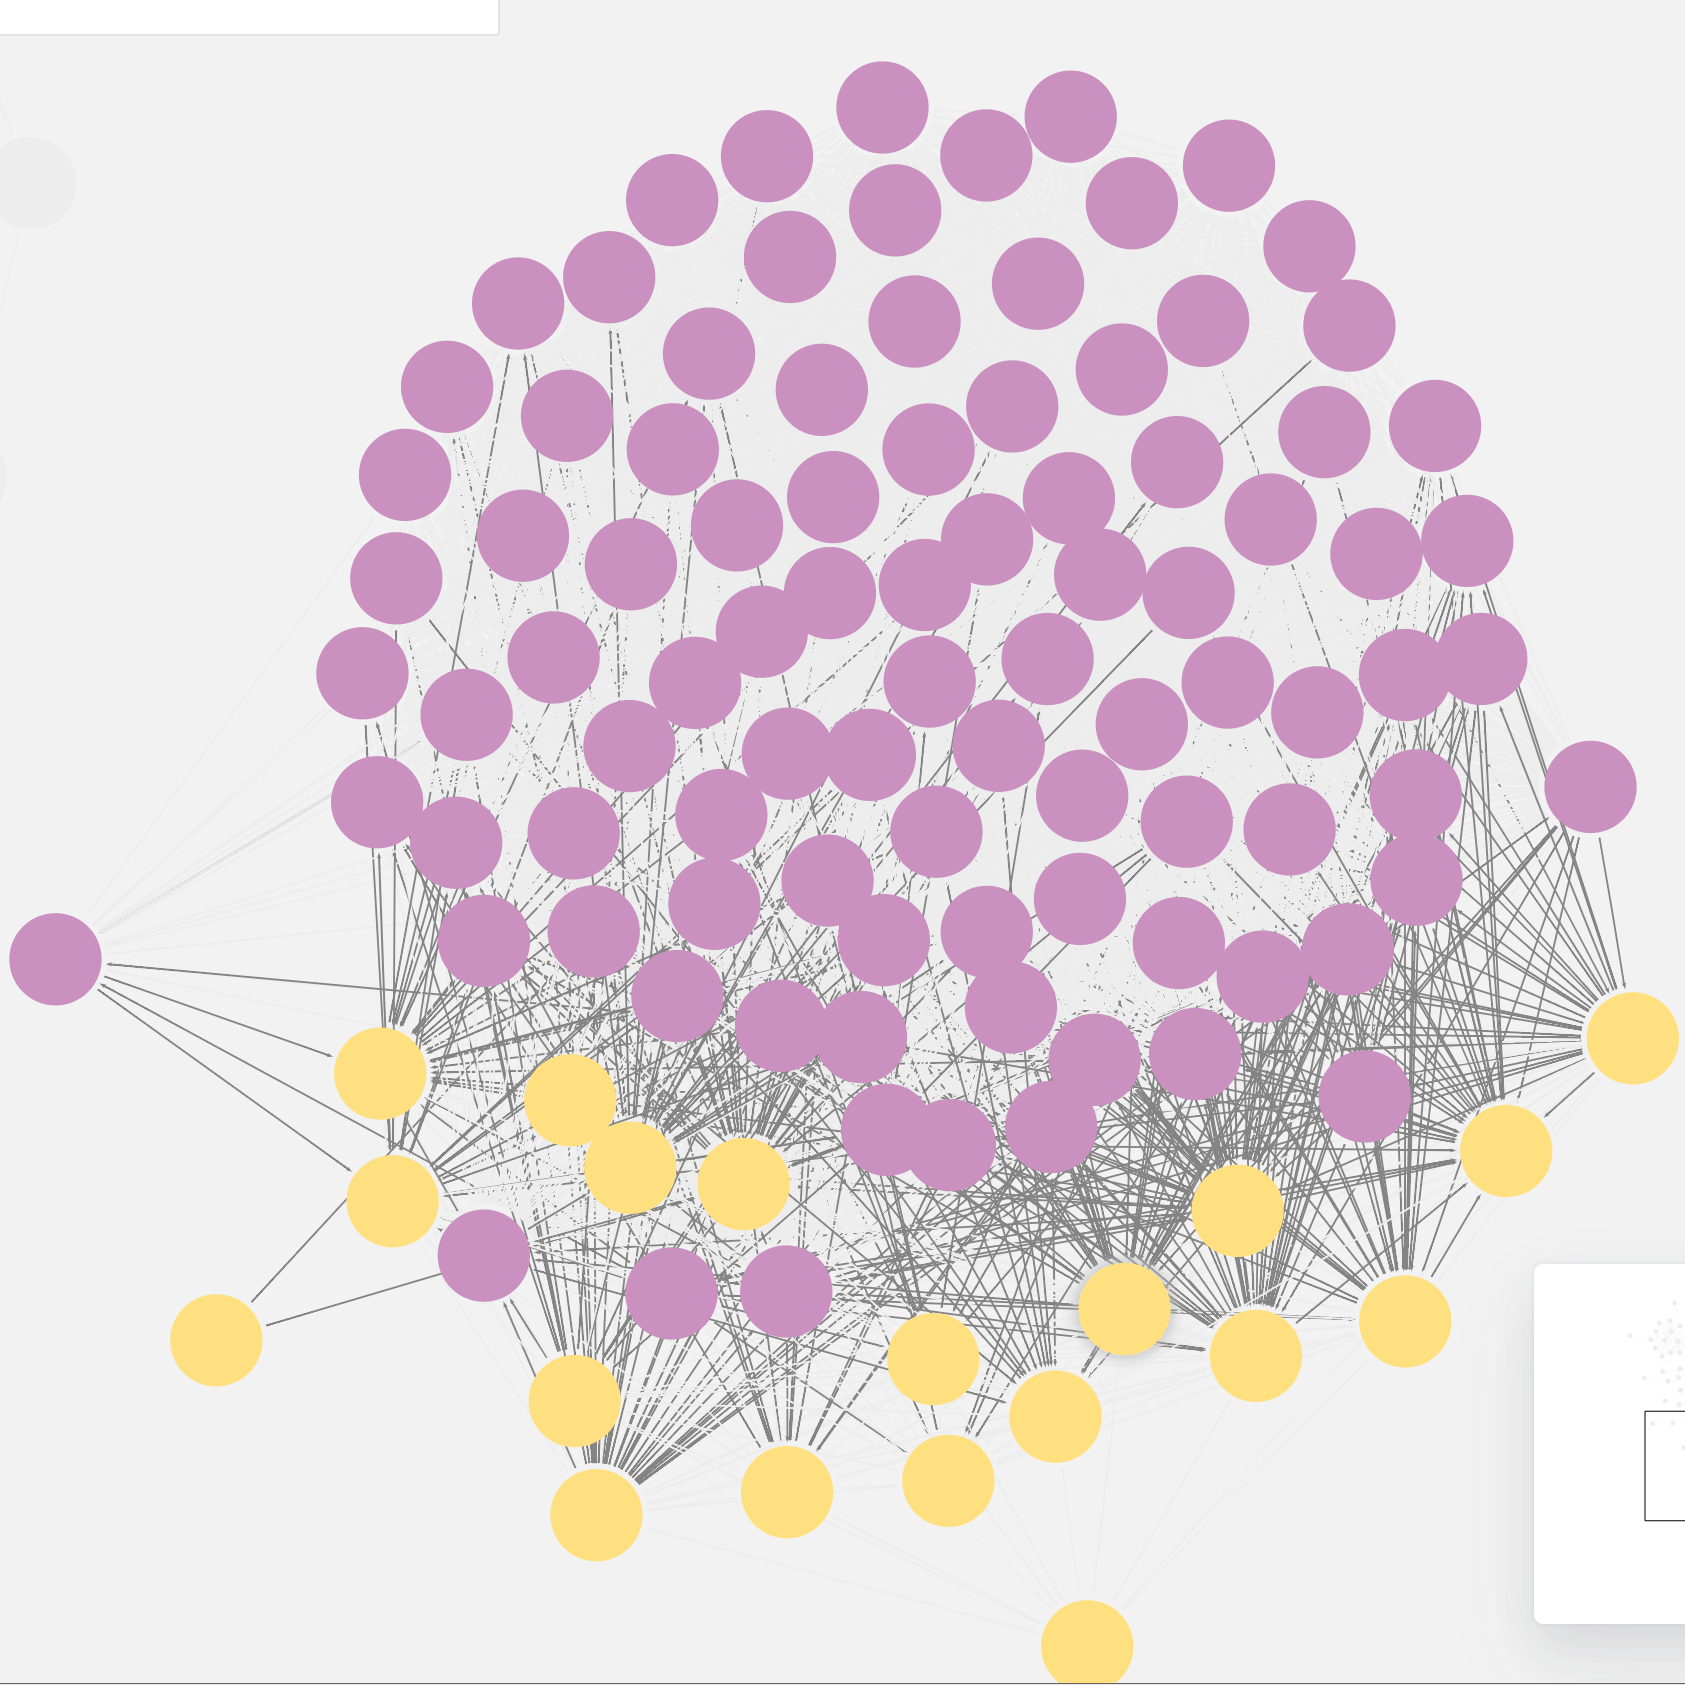
\includegraphics[width=.15\linewidth]{img/only123.png}}
    \label{subfig:ab123}
    }
  \subfigure[Graph with edges of Type 4]{
    {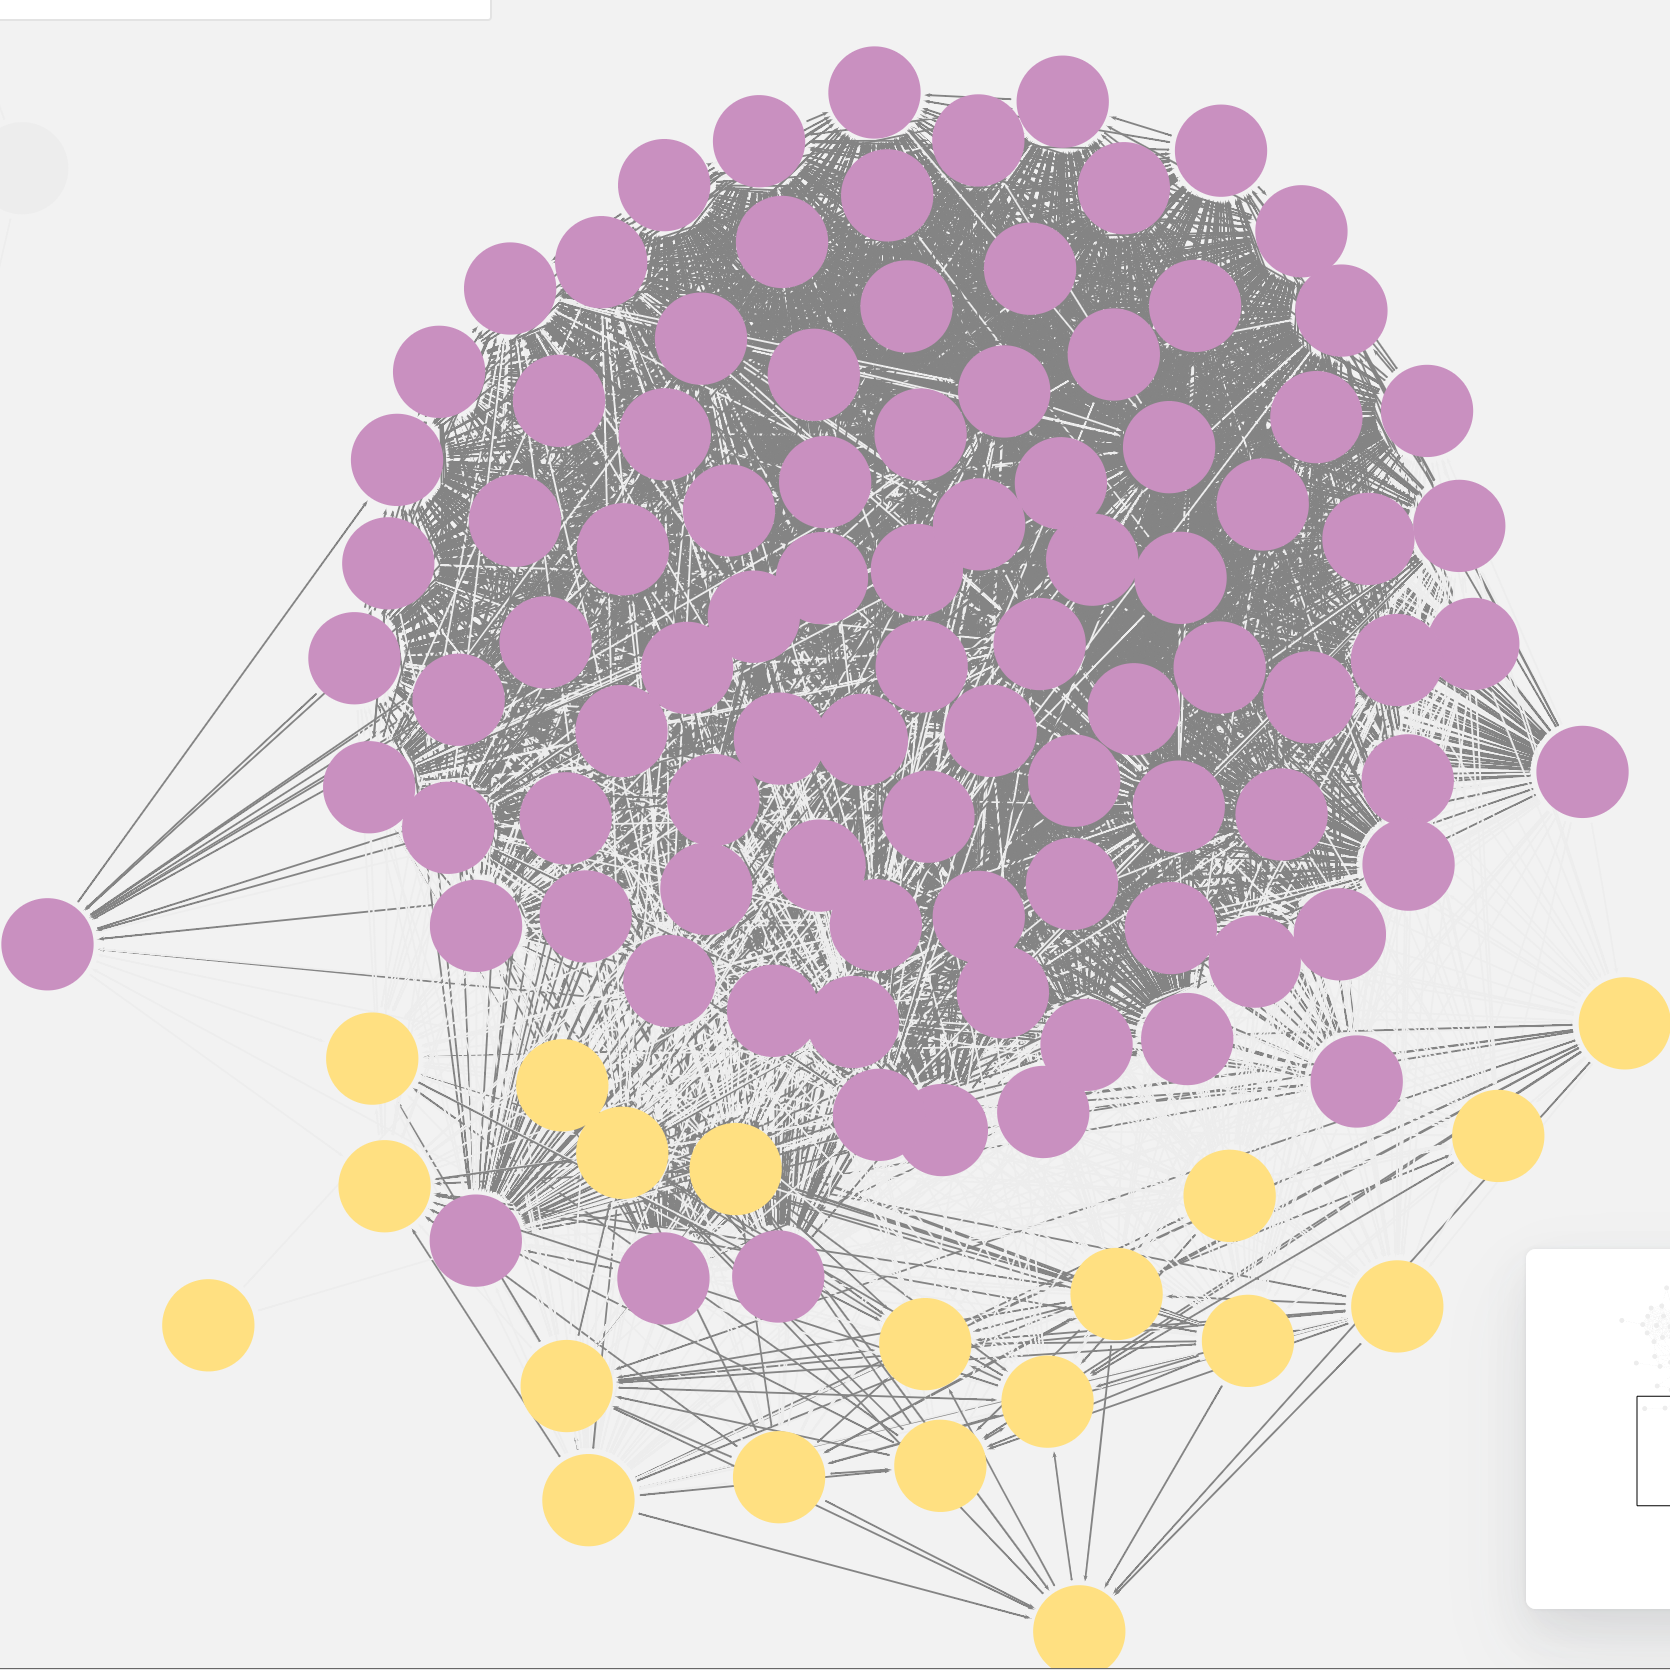
\includegraphics[width=.15\linewidth]{img/only4.png}}
    \label{subfig:ab4}
    }
  \subfigure[Graph with edges of Type 3,4]{
    {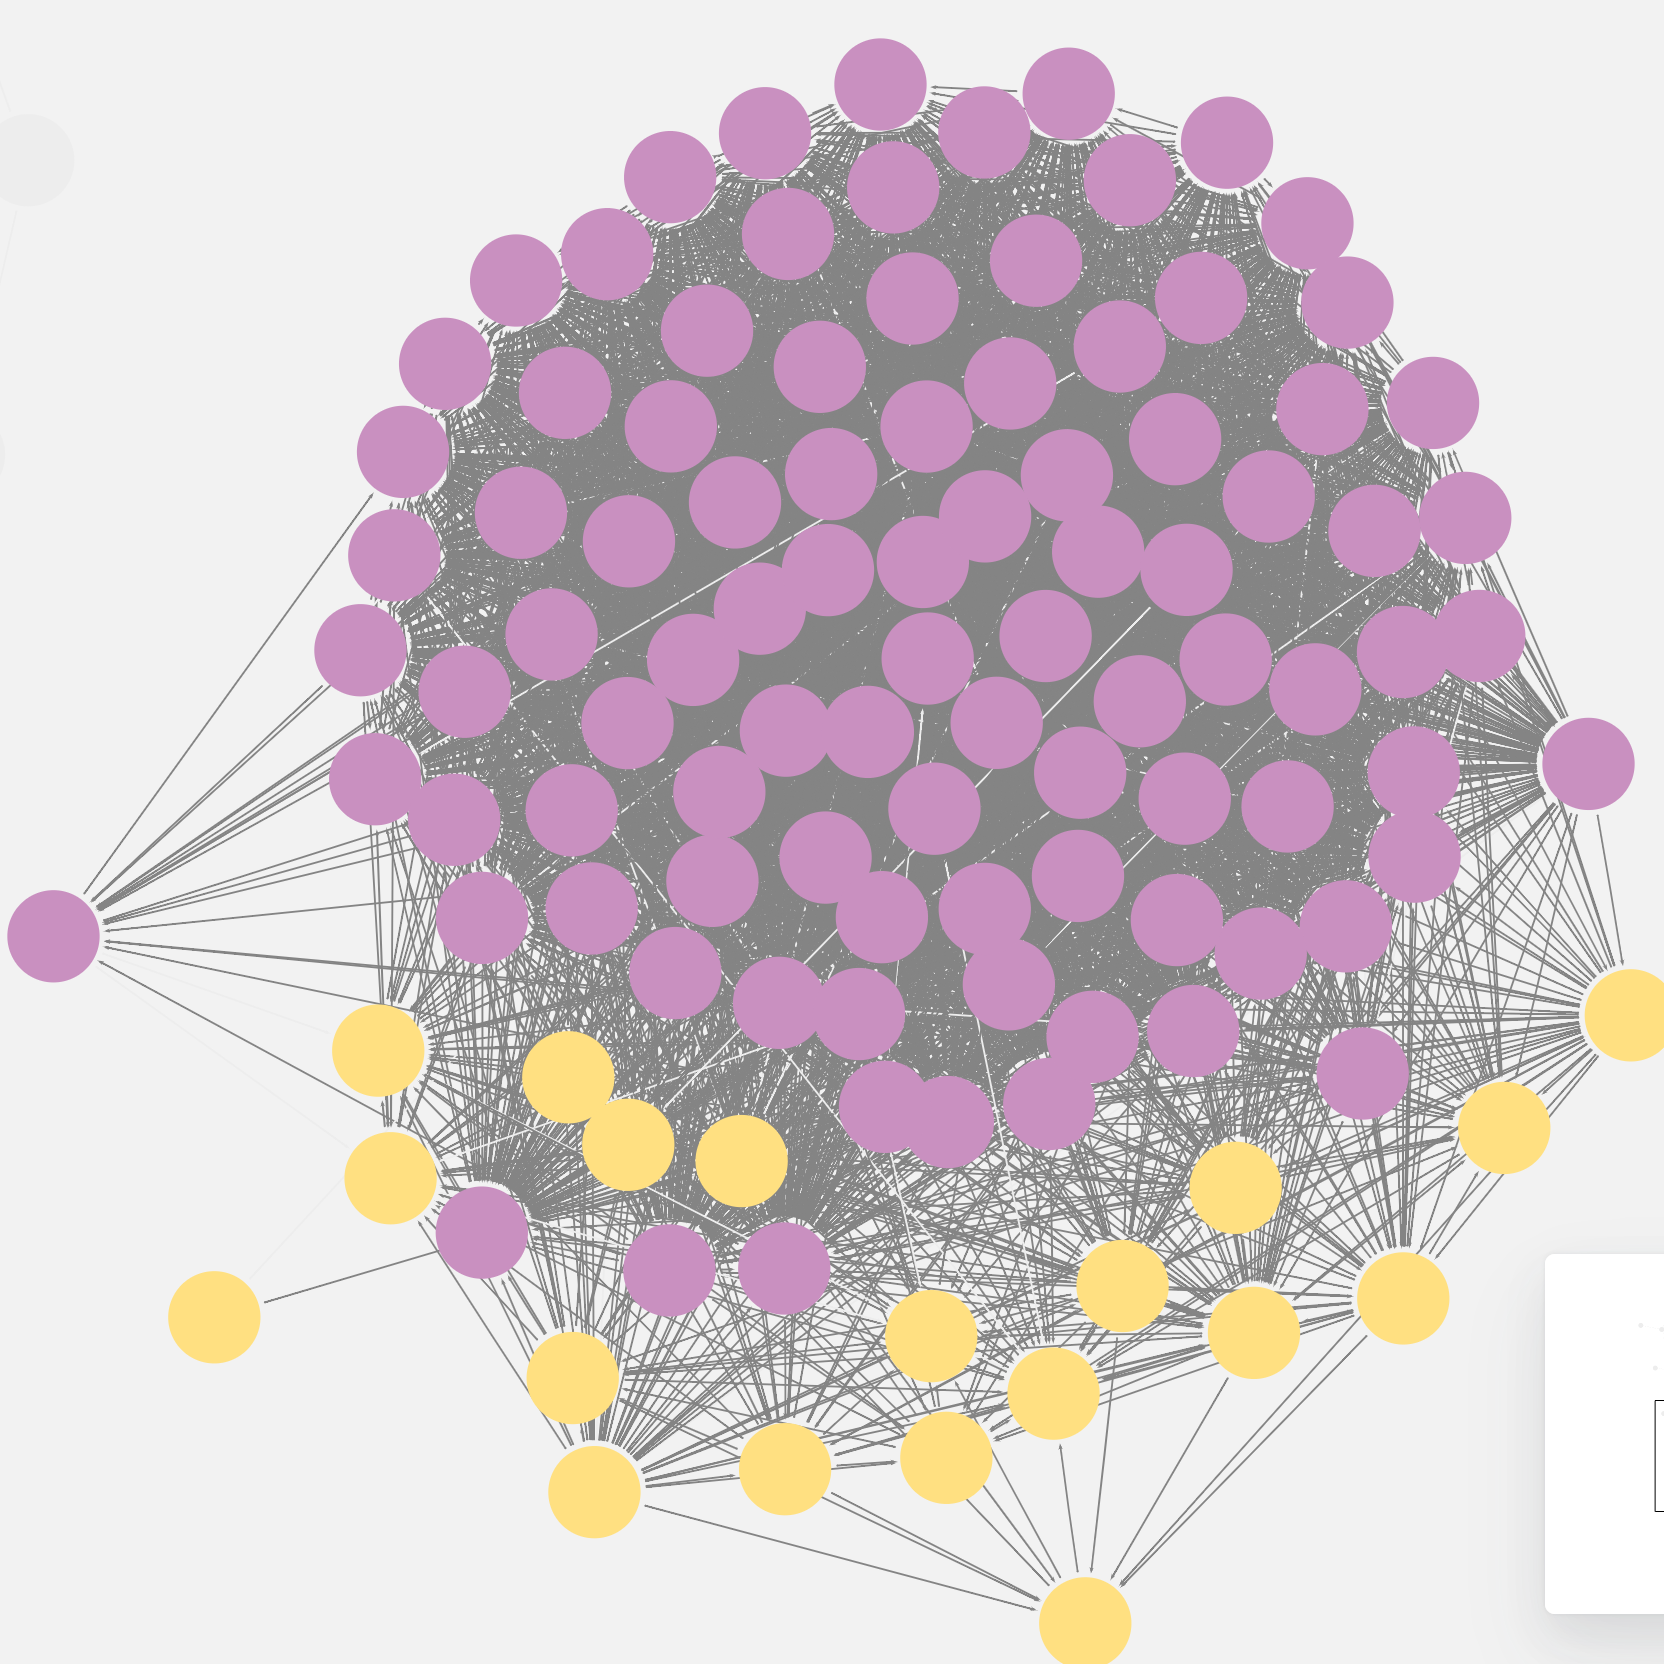
\includegraphics[width=.15\linewidth]{img/only34.png}}
    \label{subfig:ab34}
  }
  \subfigure[Graph with edges of Type 1,2]{
    {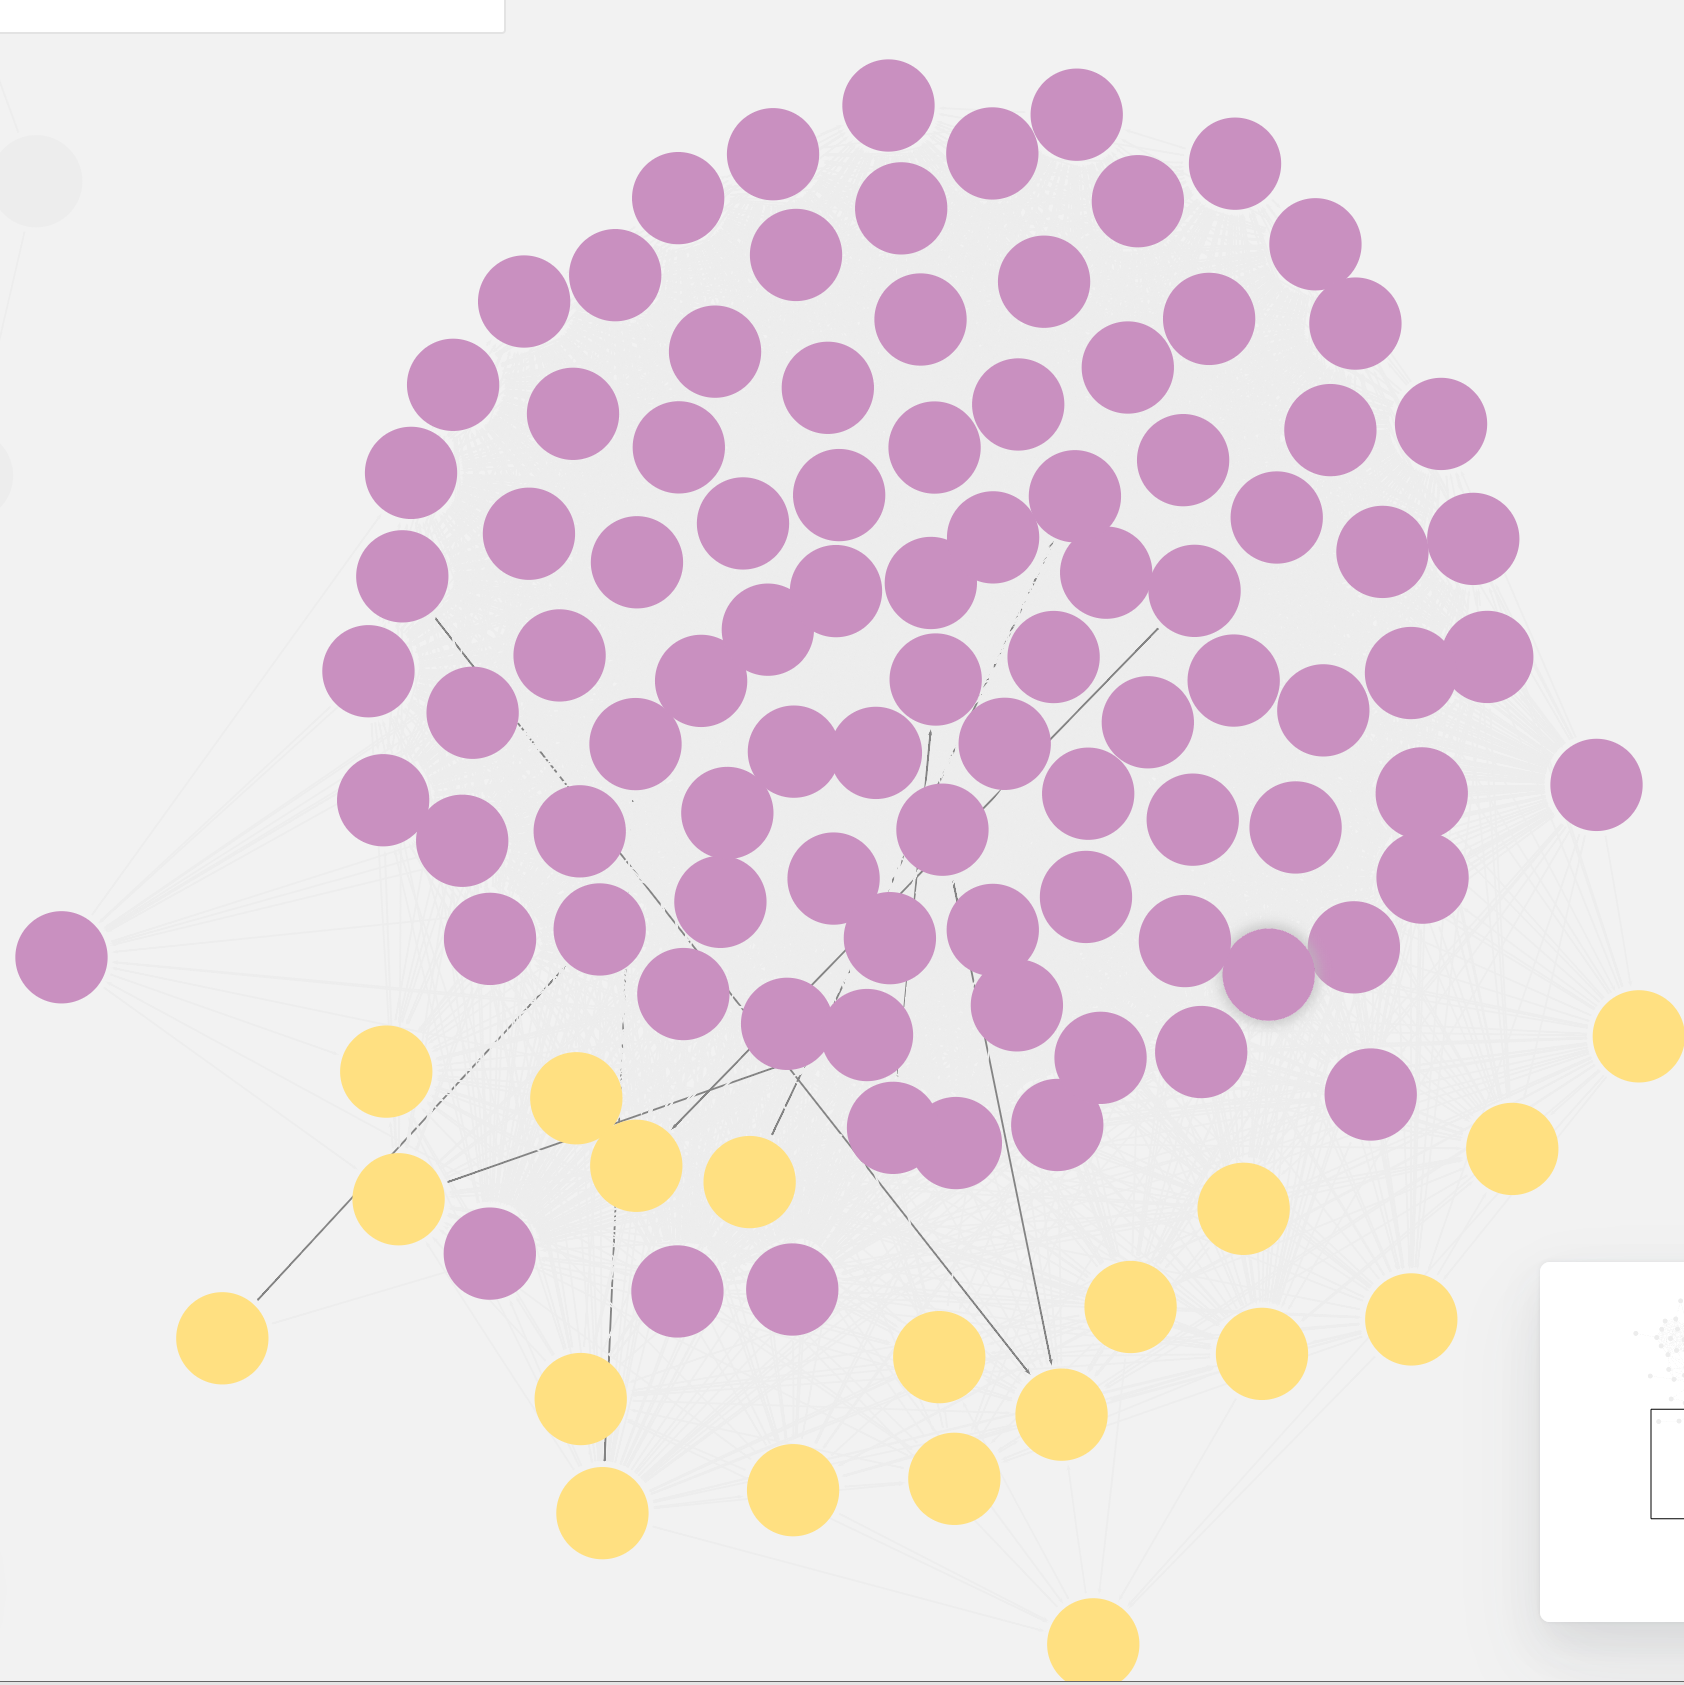
\includegraphics[width=.15\linewidth]{img/only12.png}}
    \label{subfig:ab12}
  }
  \subfigure[Graph with edges of Type 1,2,4]{
    {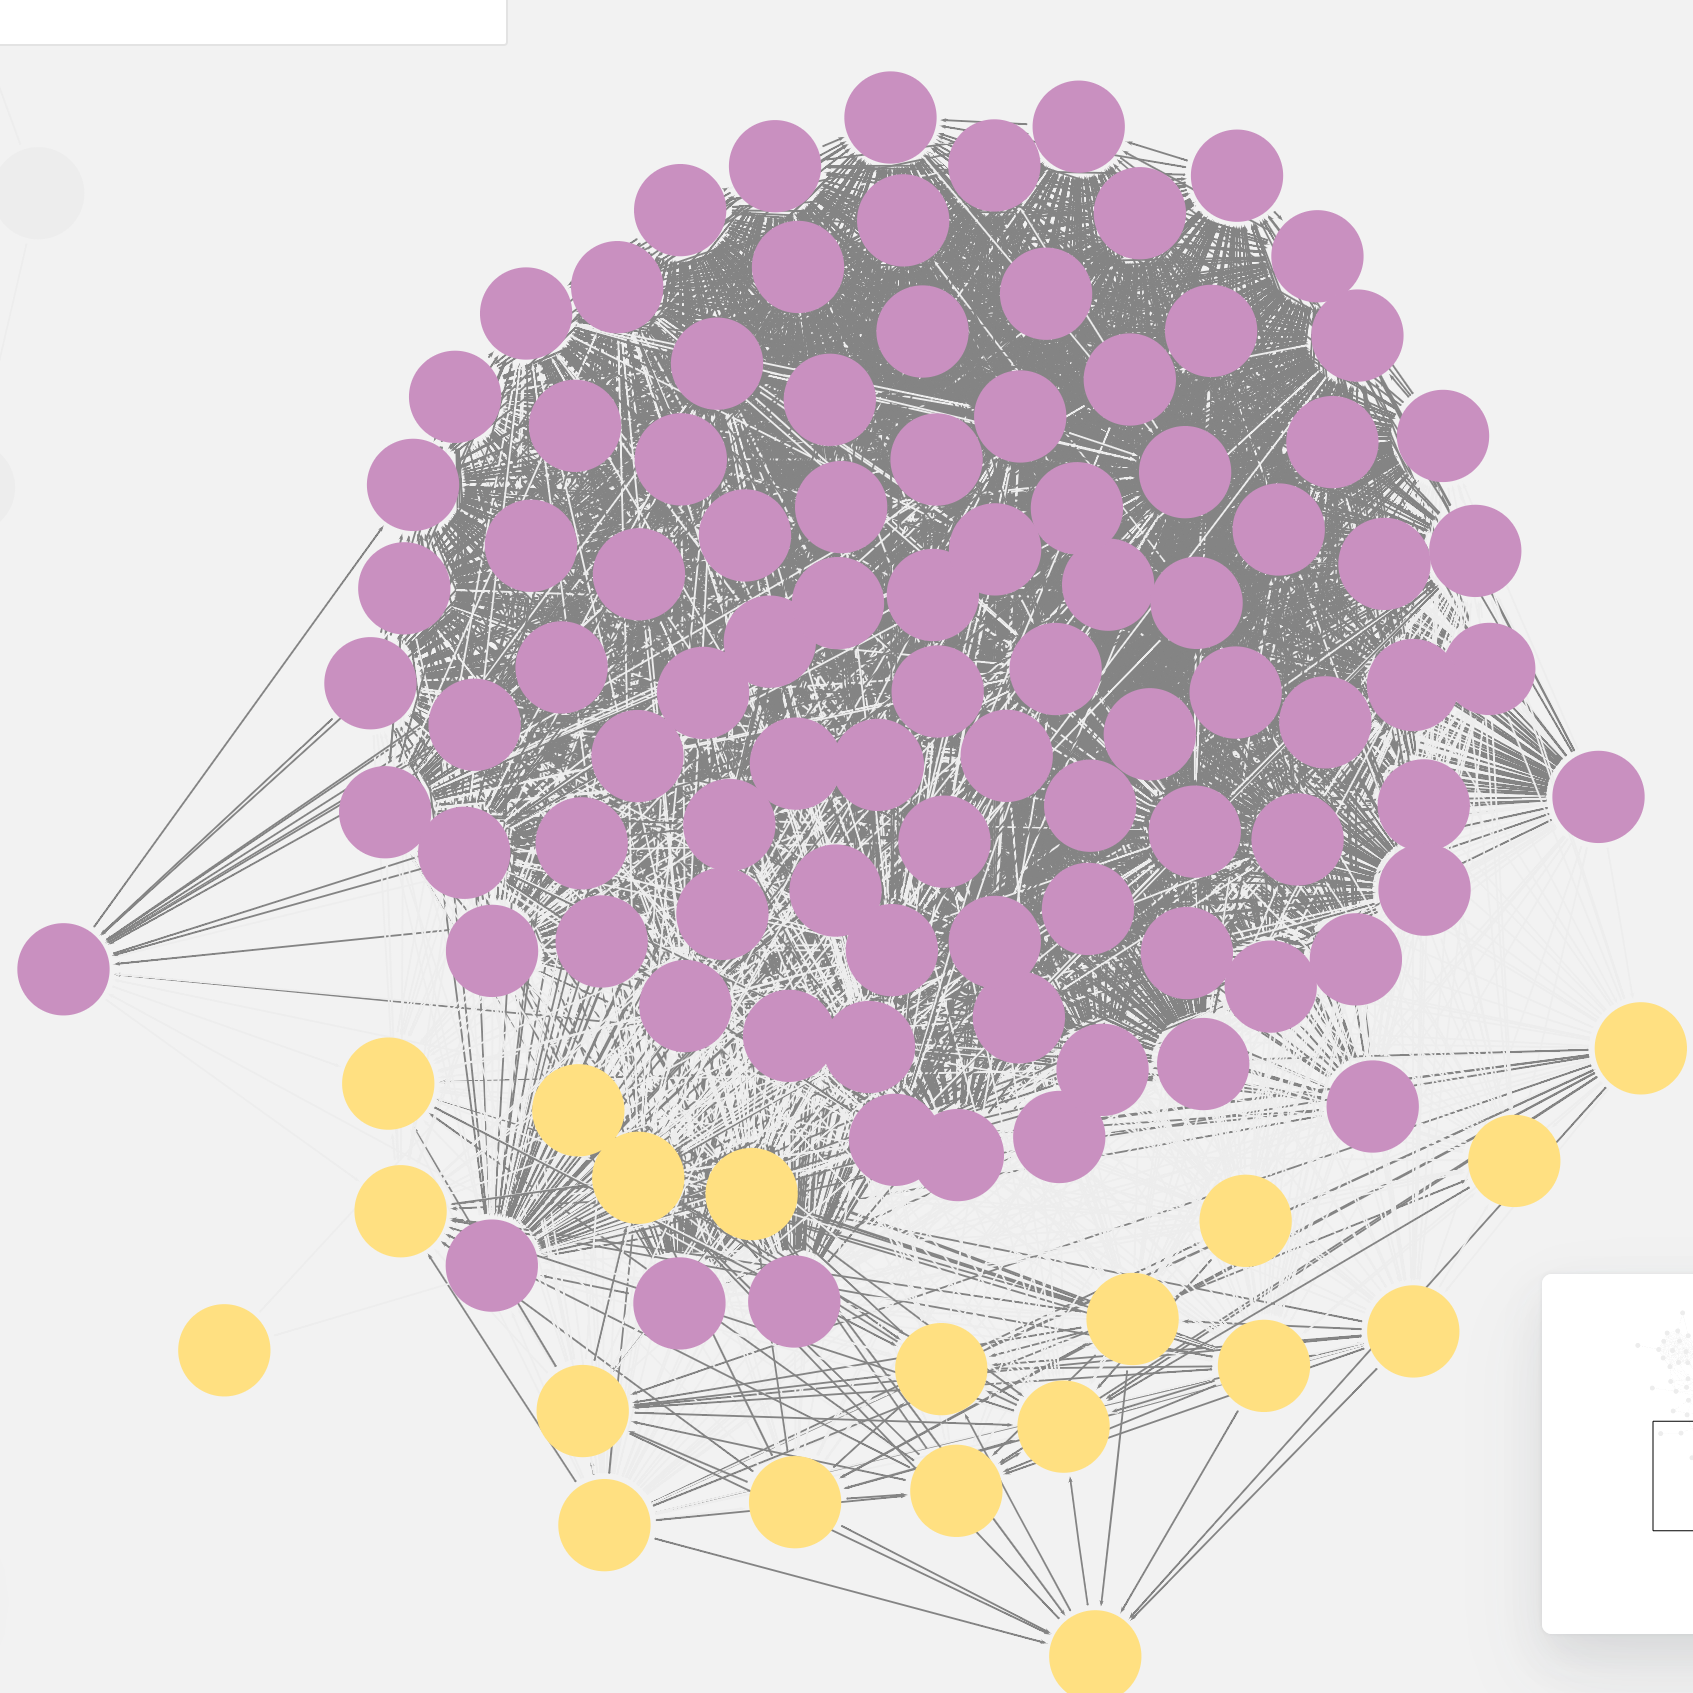
\includegraphics[width=.15\linewidth]{img/only124.png}}
    \label{subfig:ab124}
  }
  \subfigure[Graph with edges of Type 3]{
    {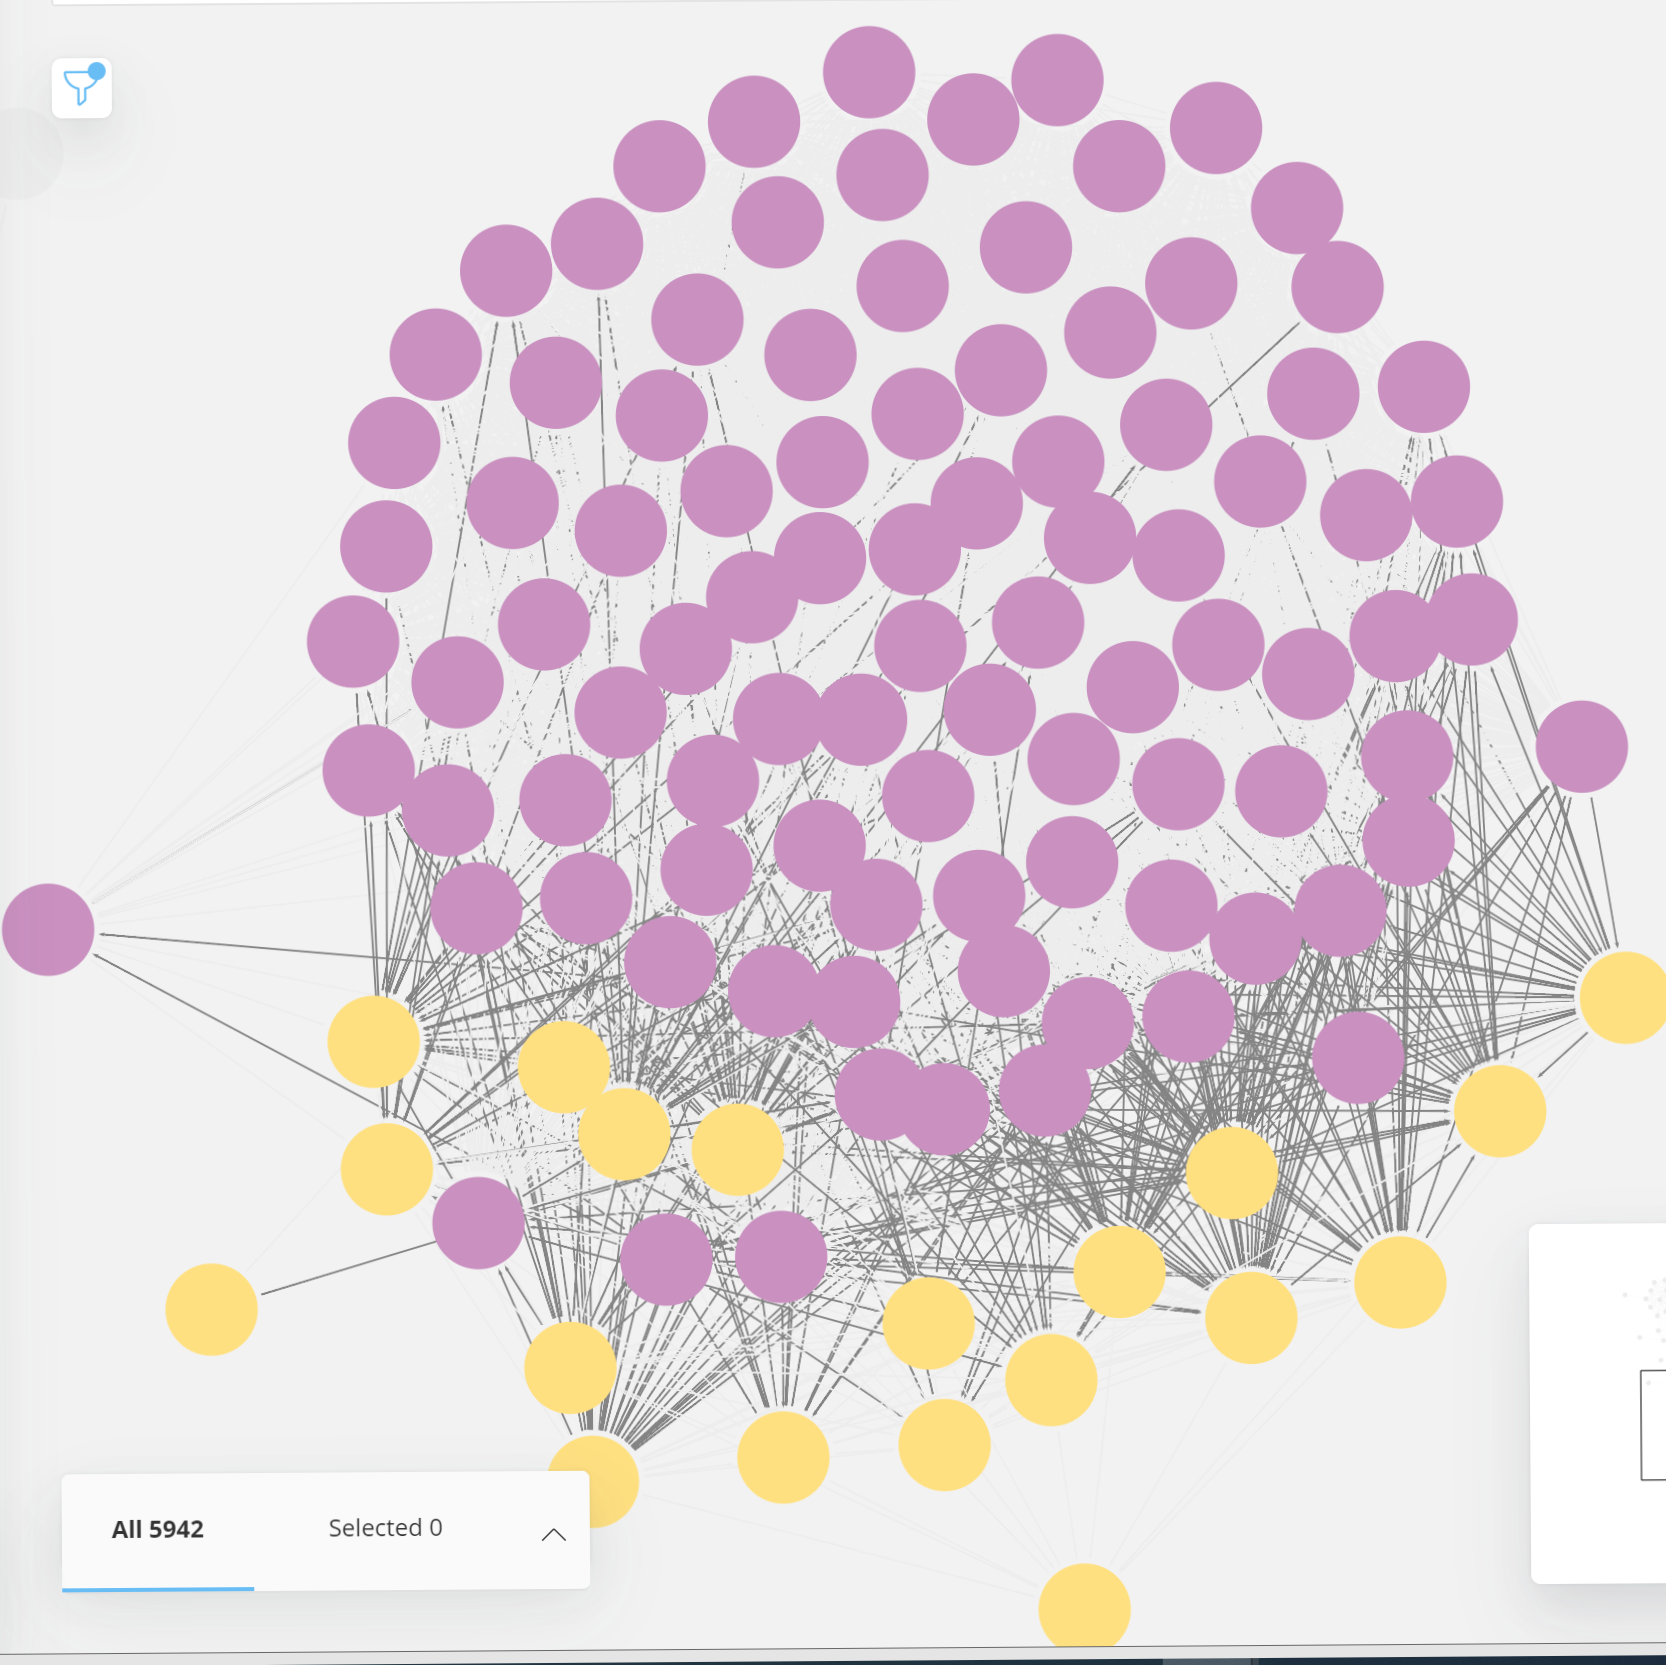
\includegraphics[width=.15\linewidth]{img/only3.png}}
    \label{subfig:ab3}
  }
    \caption{Ablation study on Relational sentence graph. {Violet nodes} are non-biased, {Yellow nodes} are biased.}
    \label{fig:ablation}
  \end{figure*}
% \begin{figure*}[!htbp]\centering
%   \begin{subfigure}[t]{.15\linewidth}
%     \resizebox{\linewidth}{!}{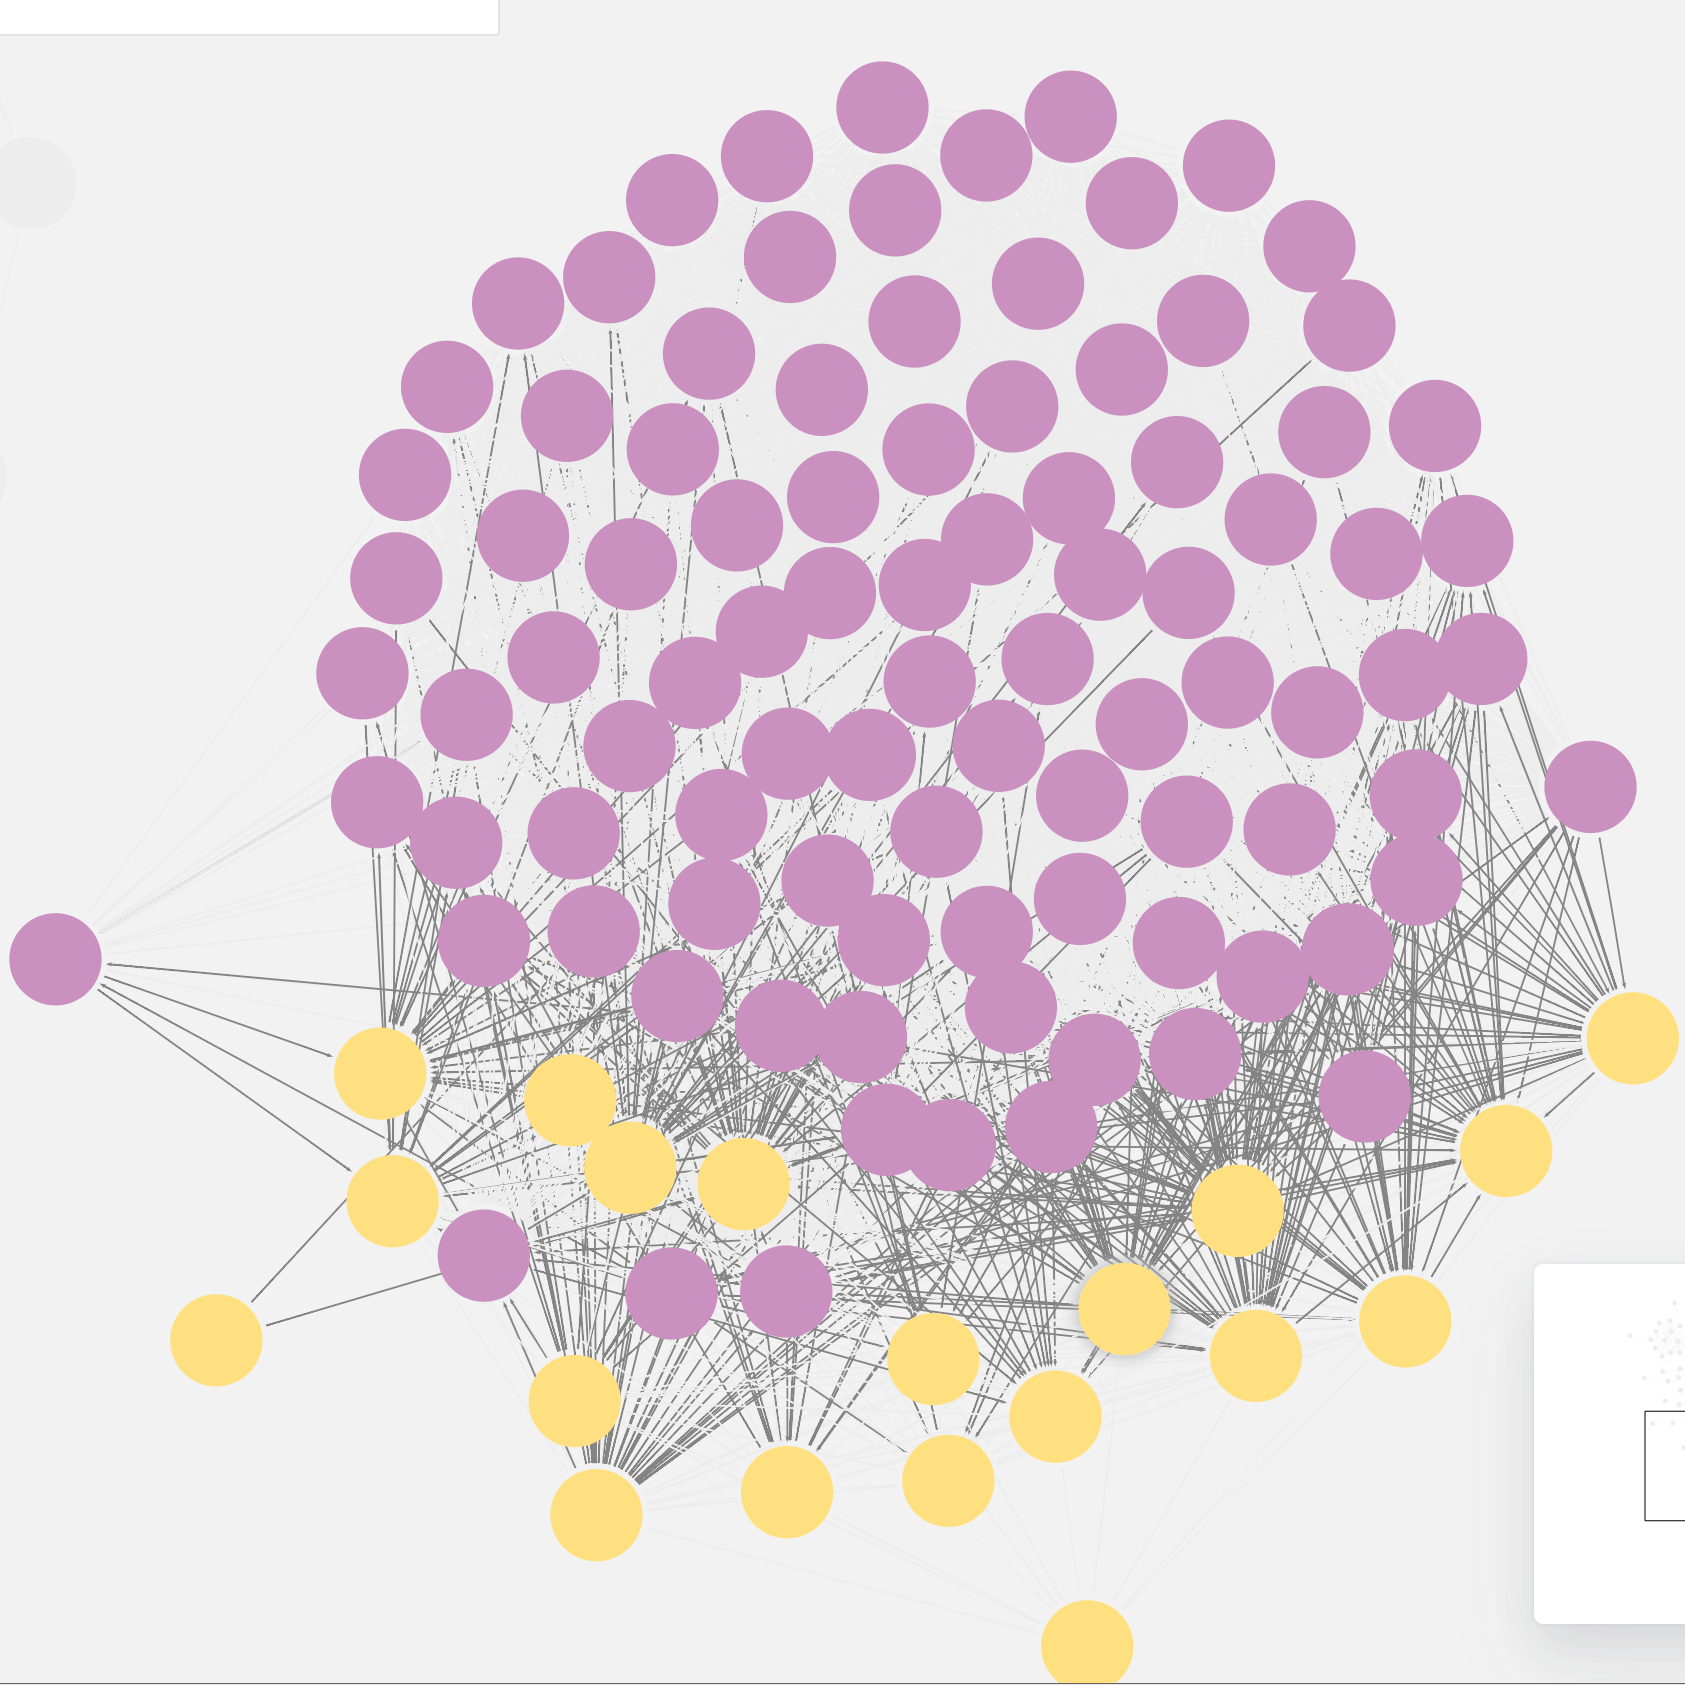
\includegraphics[]{img/only123.png}}
%     \caption{ Graph with edges of Type 1,2,3}
%     \label{subfig:ab123}
%   \end{subfigure}
%   \begin{subfigure}[t]{.15\linewidth}
%     \resizebox{\linewidth}{!}{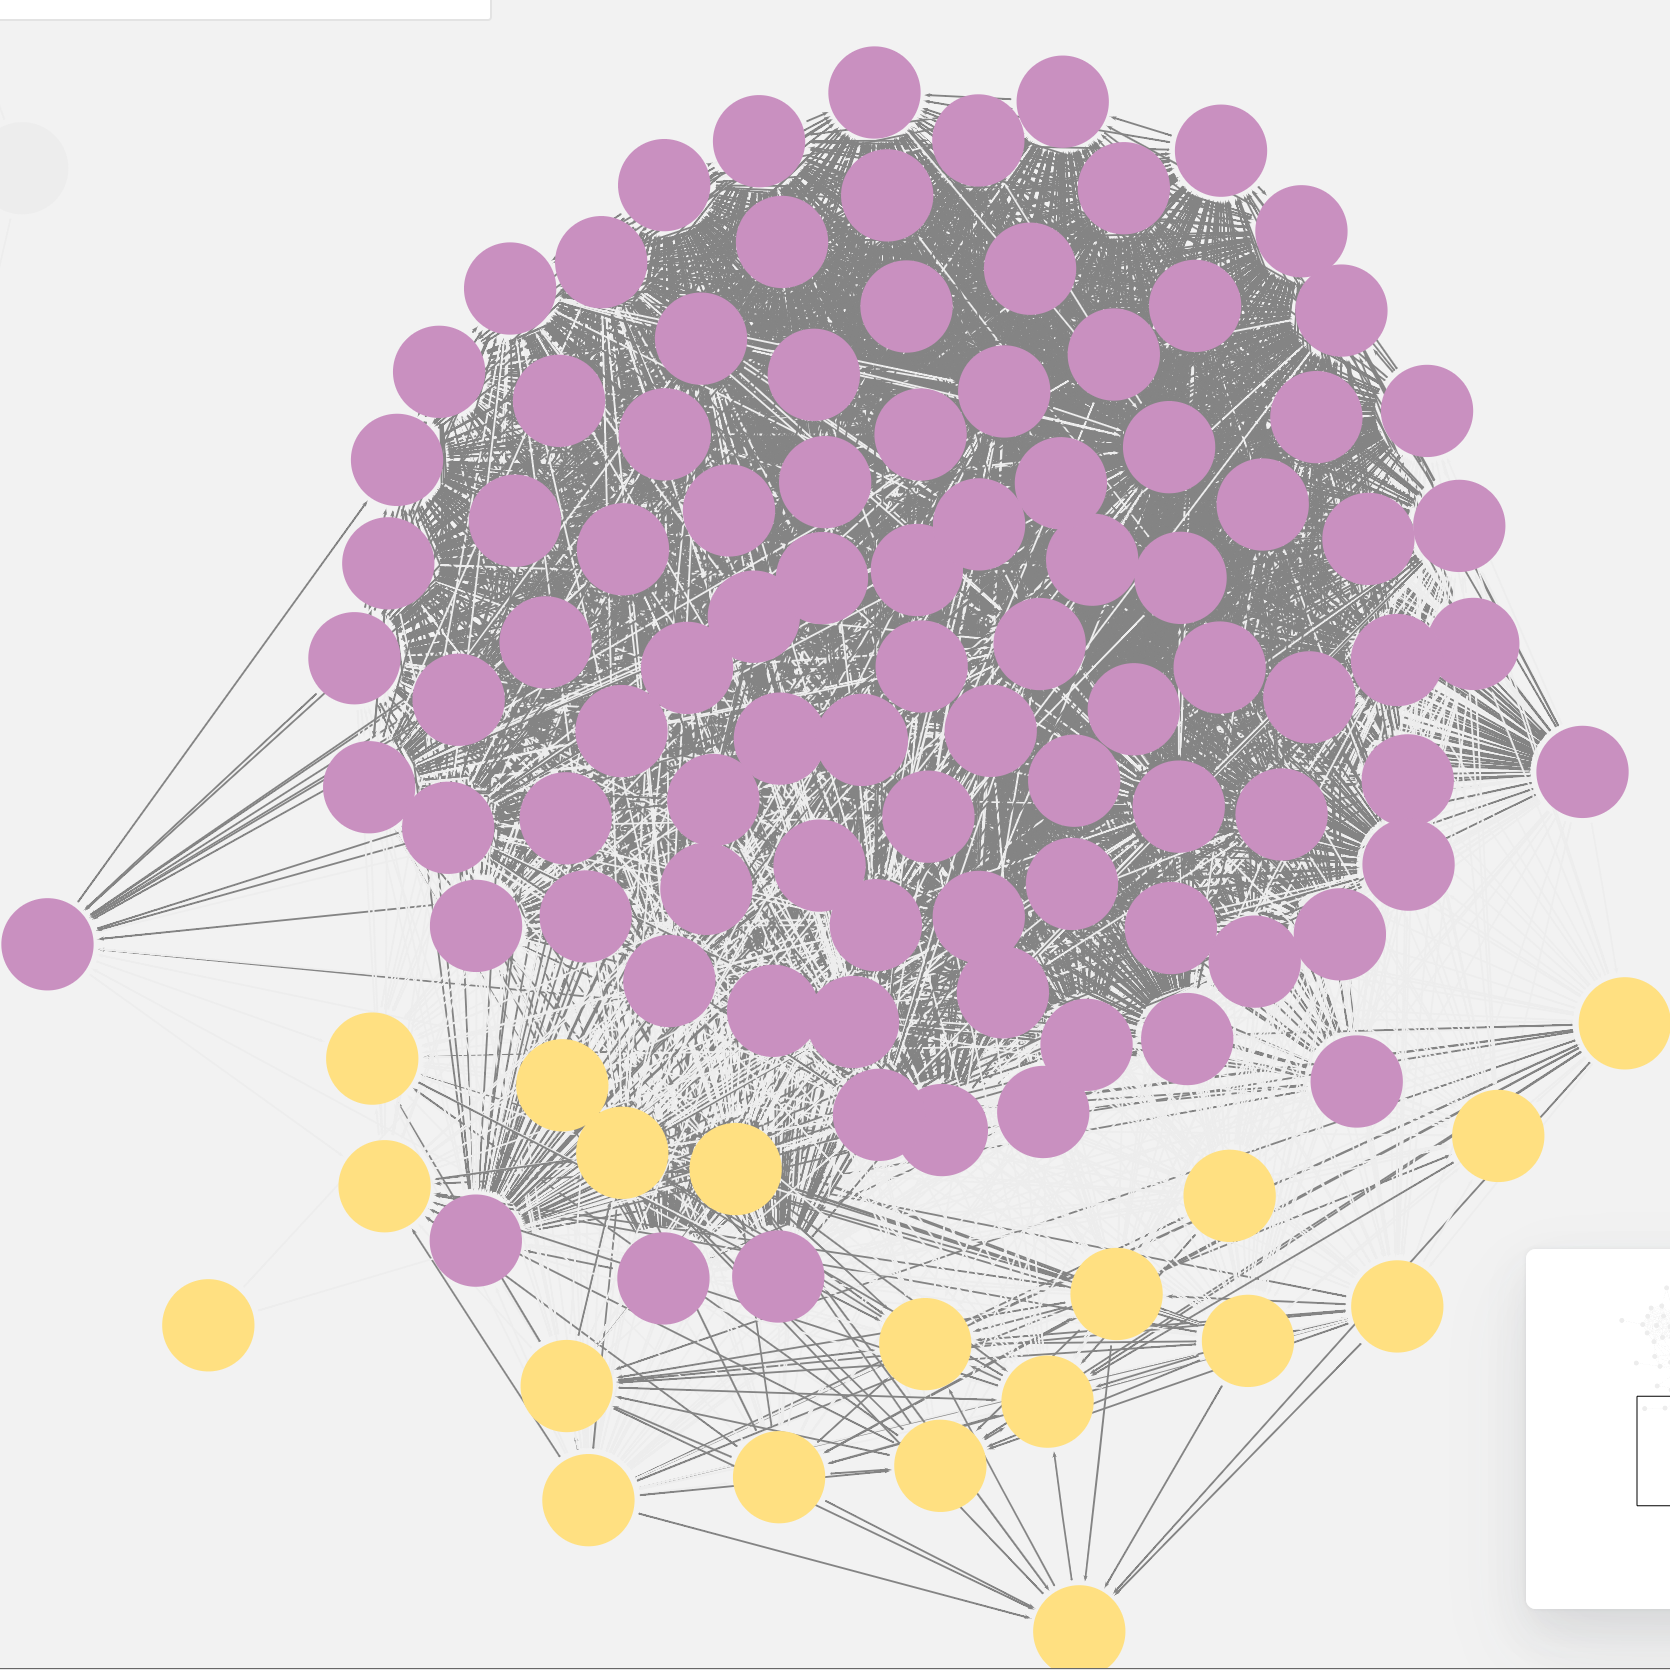
\includegraphics[]{img/only4.png}}
%     \caption{ Graph with edges of Type 4}
%     \label{subfig:ab4}
%   \end{subfigure}
%   \begin{subfigure}[t]{.15\linewidth}
%     \resizebox{\linewidth}{!}{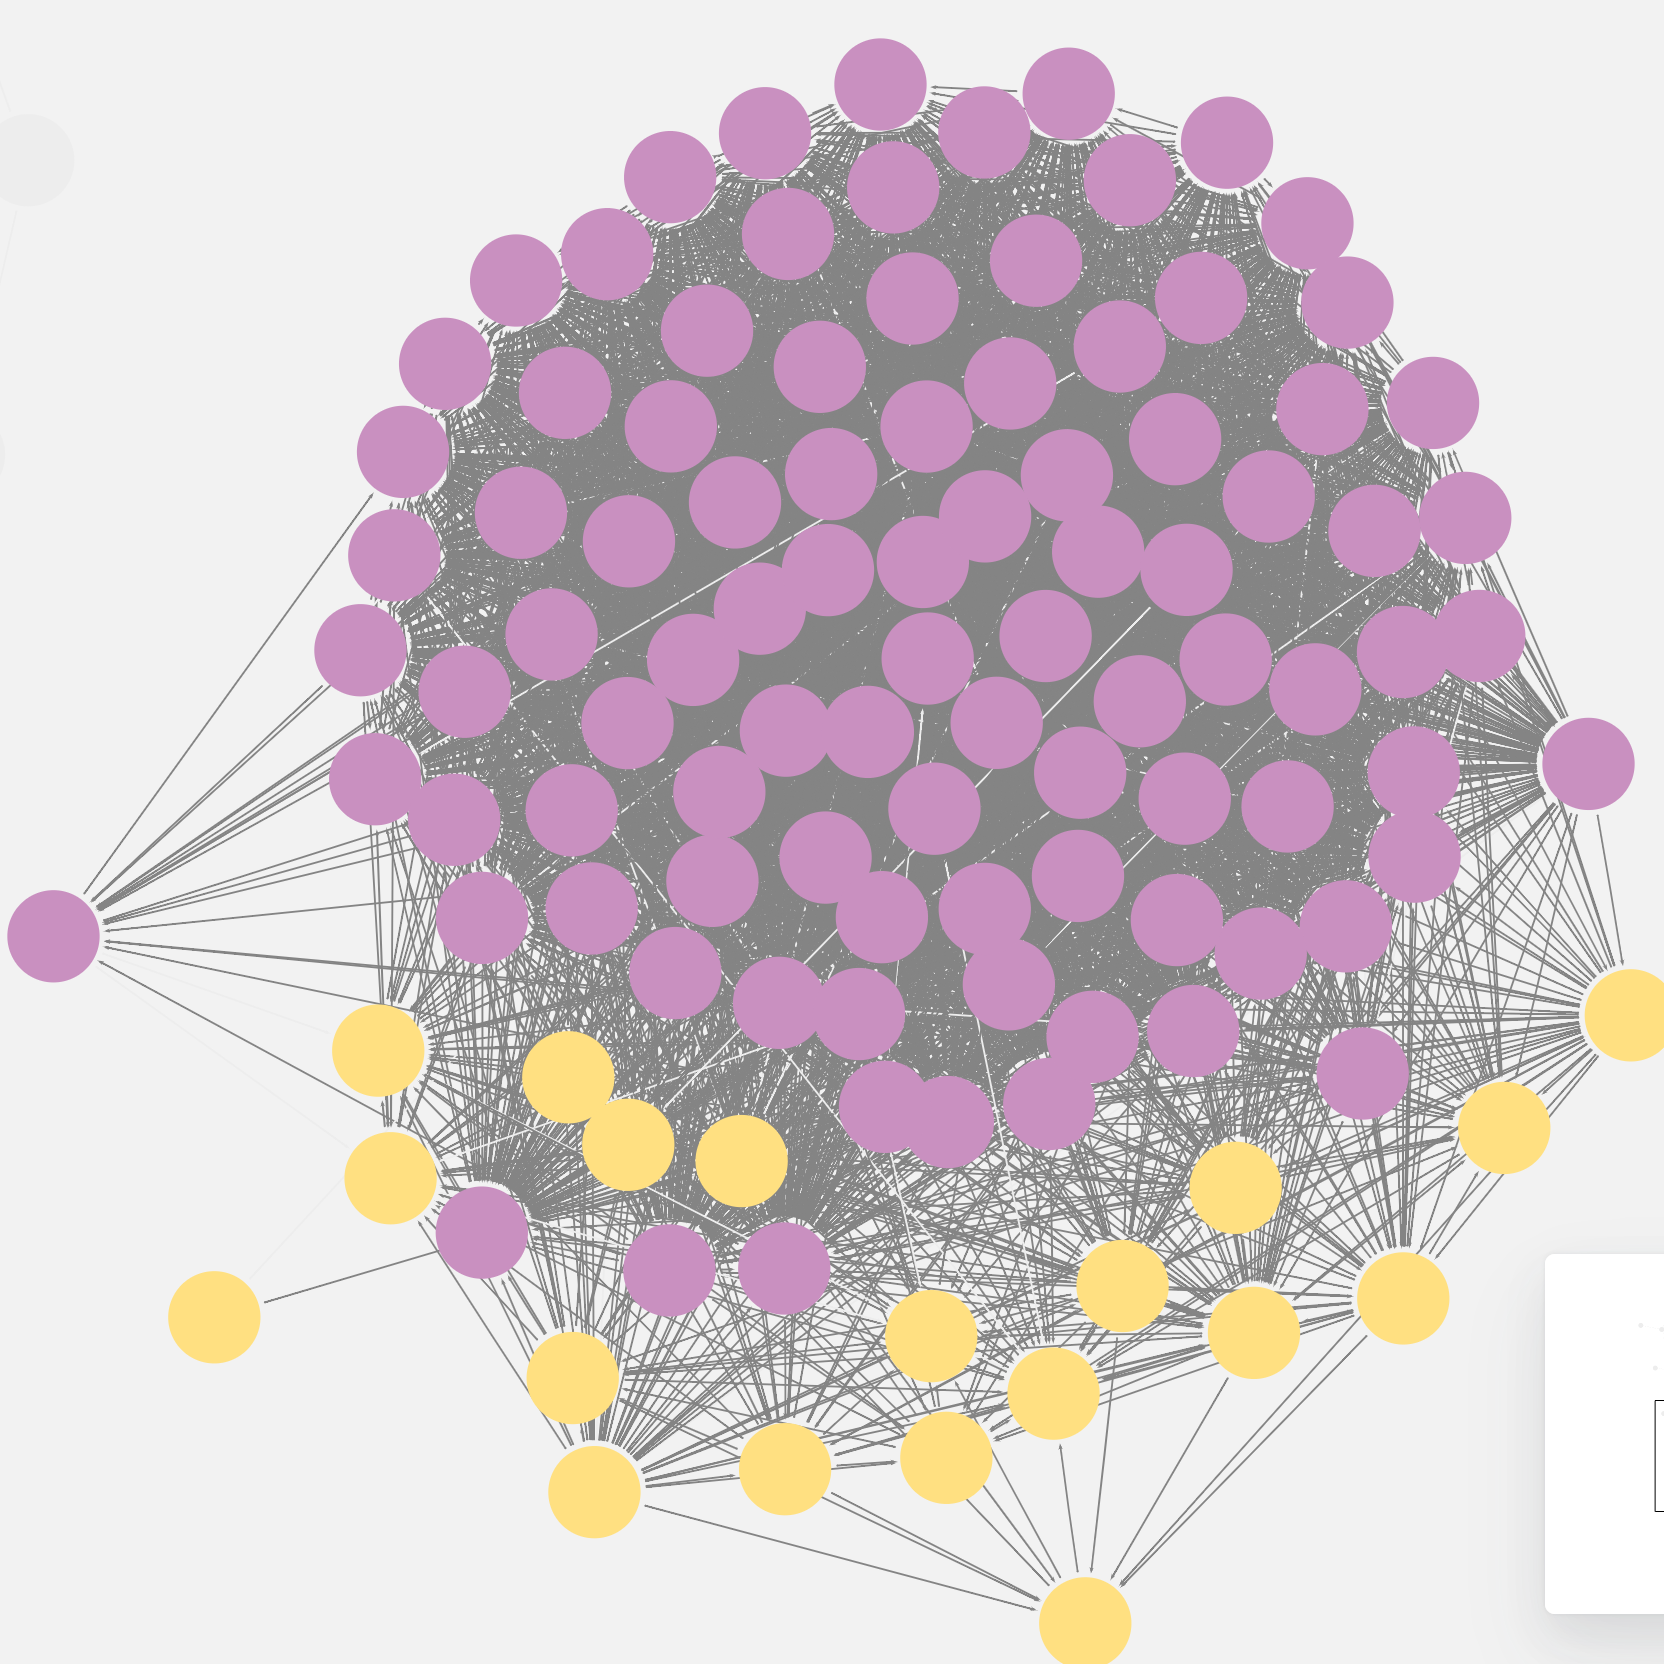
\includegraphics[]{img/only34.png}}
%     \caption{ Graph with edges of Type 3,4}
%     \label{subfig:ab34}
%   \end{subfigure}
%   \begin{subfigure}[t]{.15\linewidth}
%     \resizebox{\linewidth}{!}{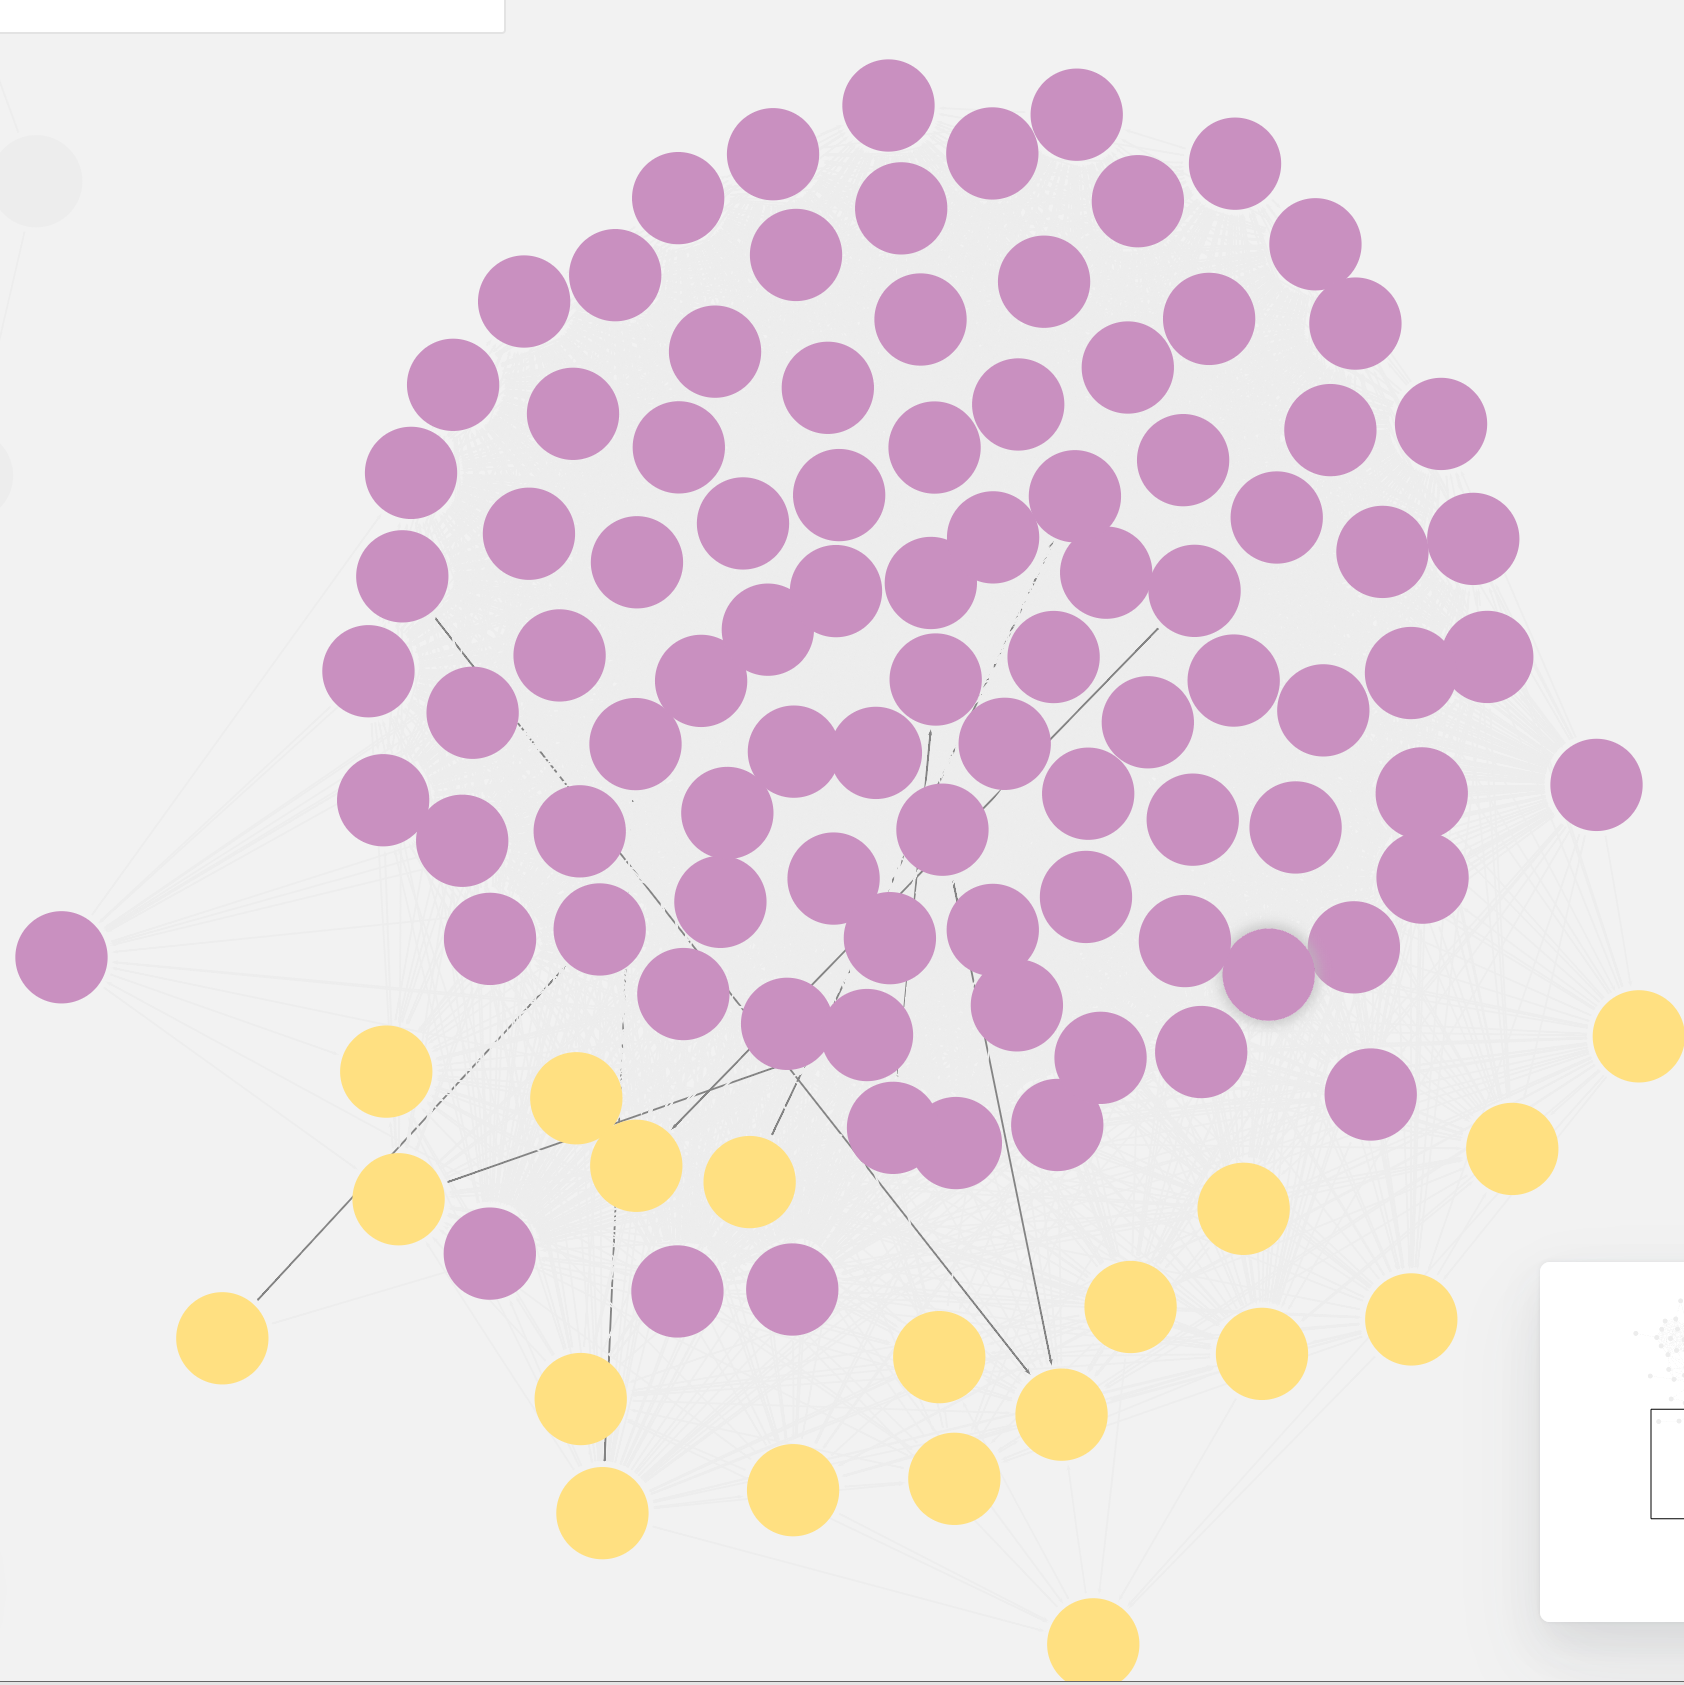
\includegraphics[]{img/only12.png}}
%     \caption{ Graph with edges of Type 1,2}
%     \label{subfig:ab12}
%   \end{subfigure}
%   \begin{subfigure}[t]{.15\linewidth}
%     \resizebox{\linewidth}{!}{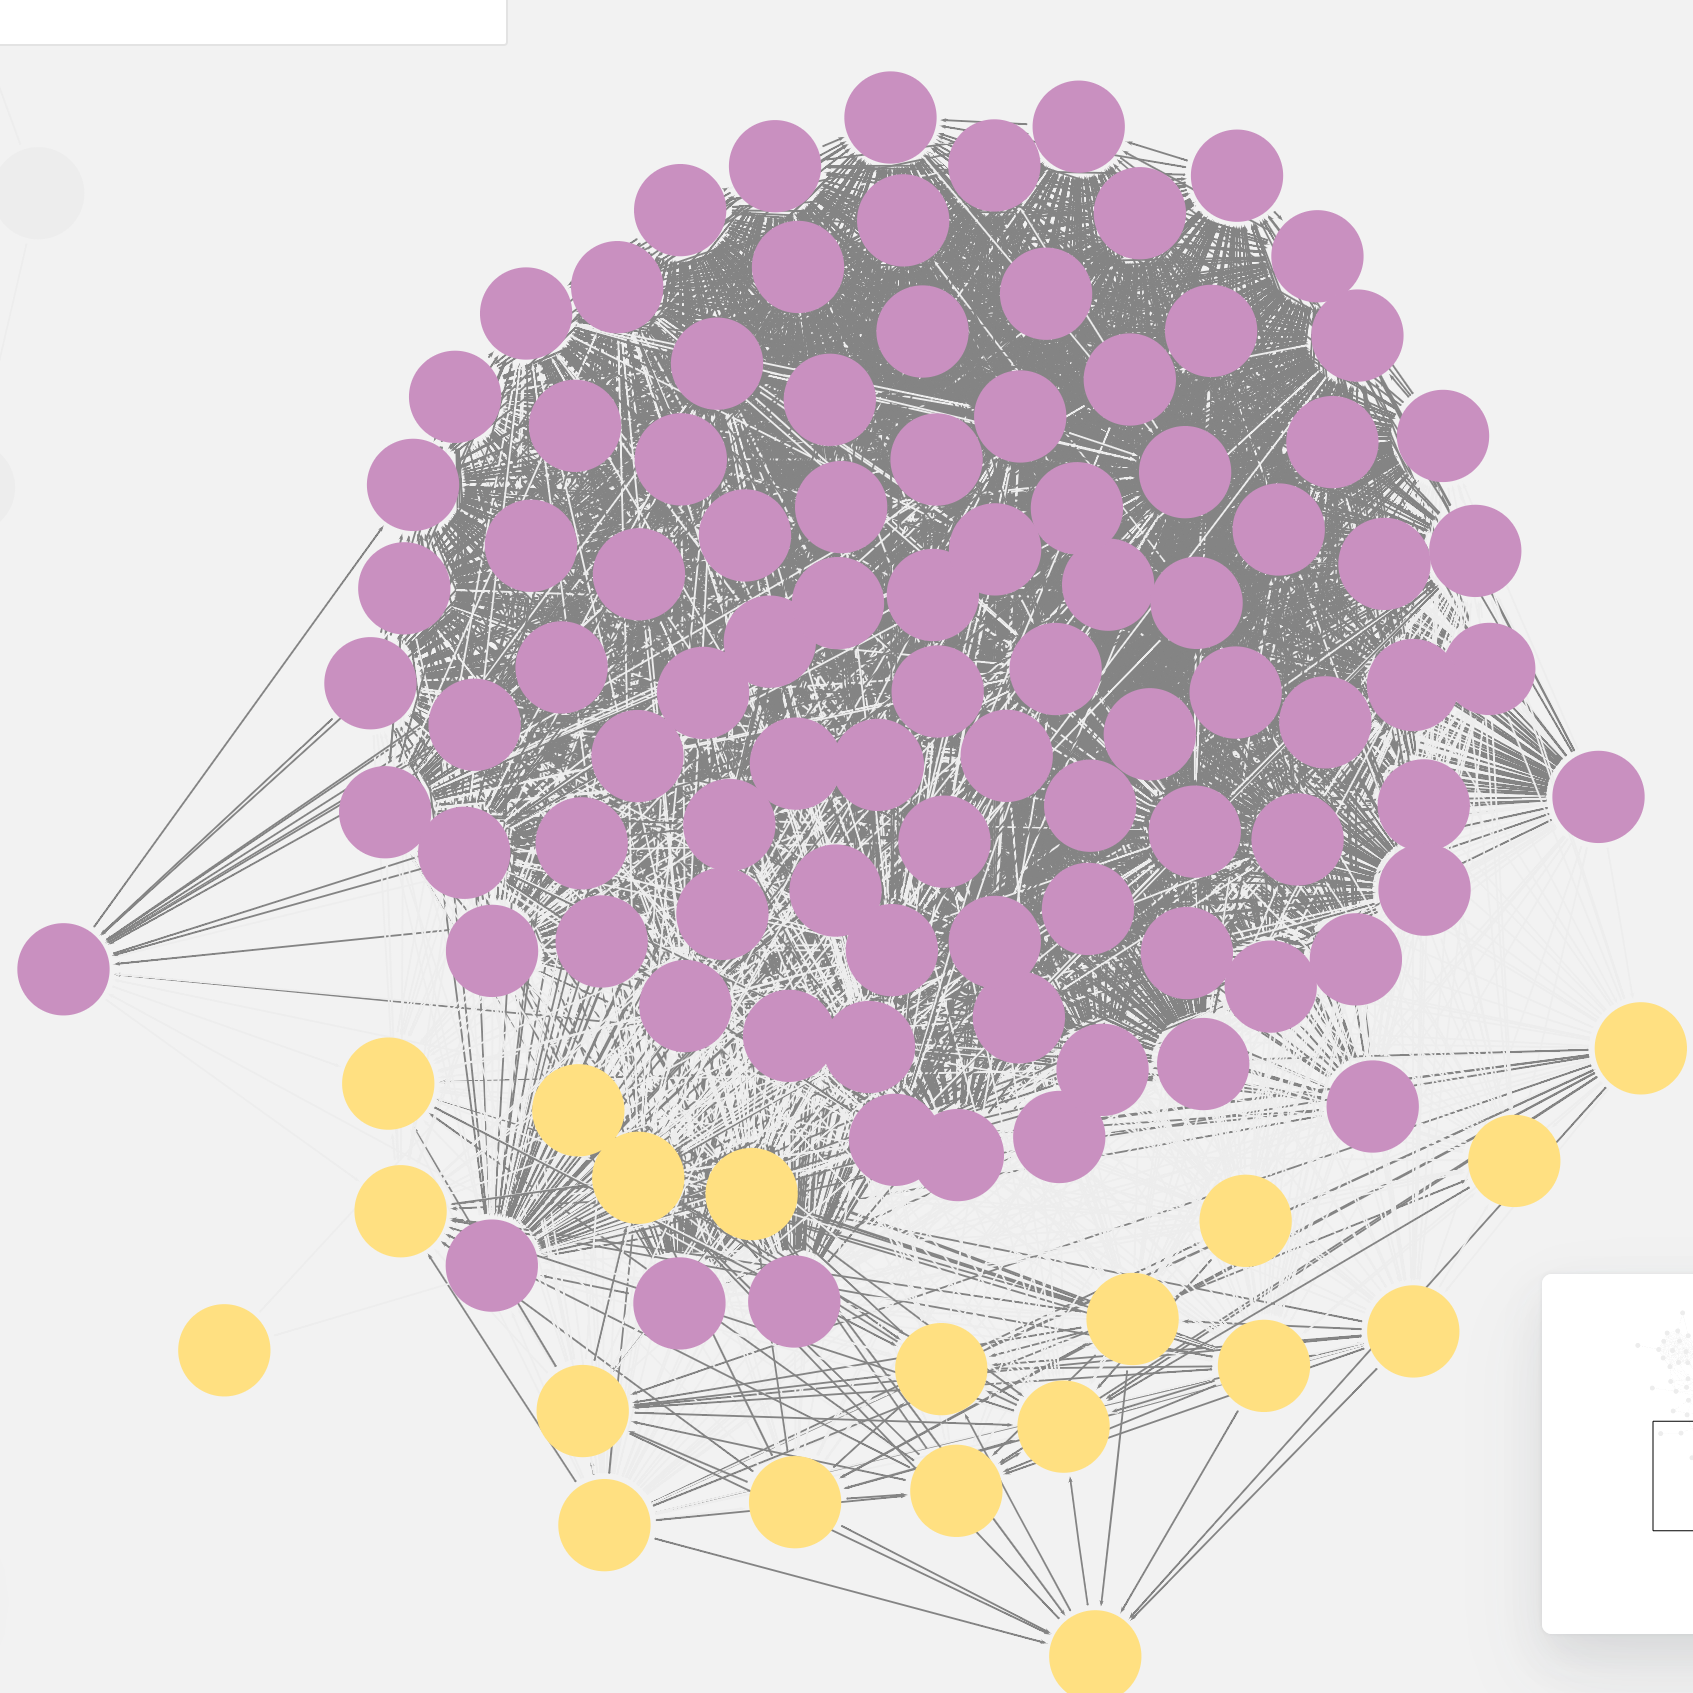
\includegraphics[]{img/only124.png}}
%     \caption{ Graph with edges of Type 1,2,4}
%     \label{subfig:ab124}
%   \end{subfigure}
%   \begin{subfigure}[t]{.15\linewidth}
%     \resizebox{\linewidth}{!}{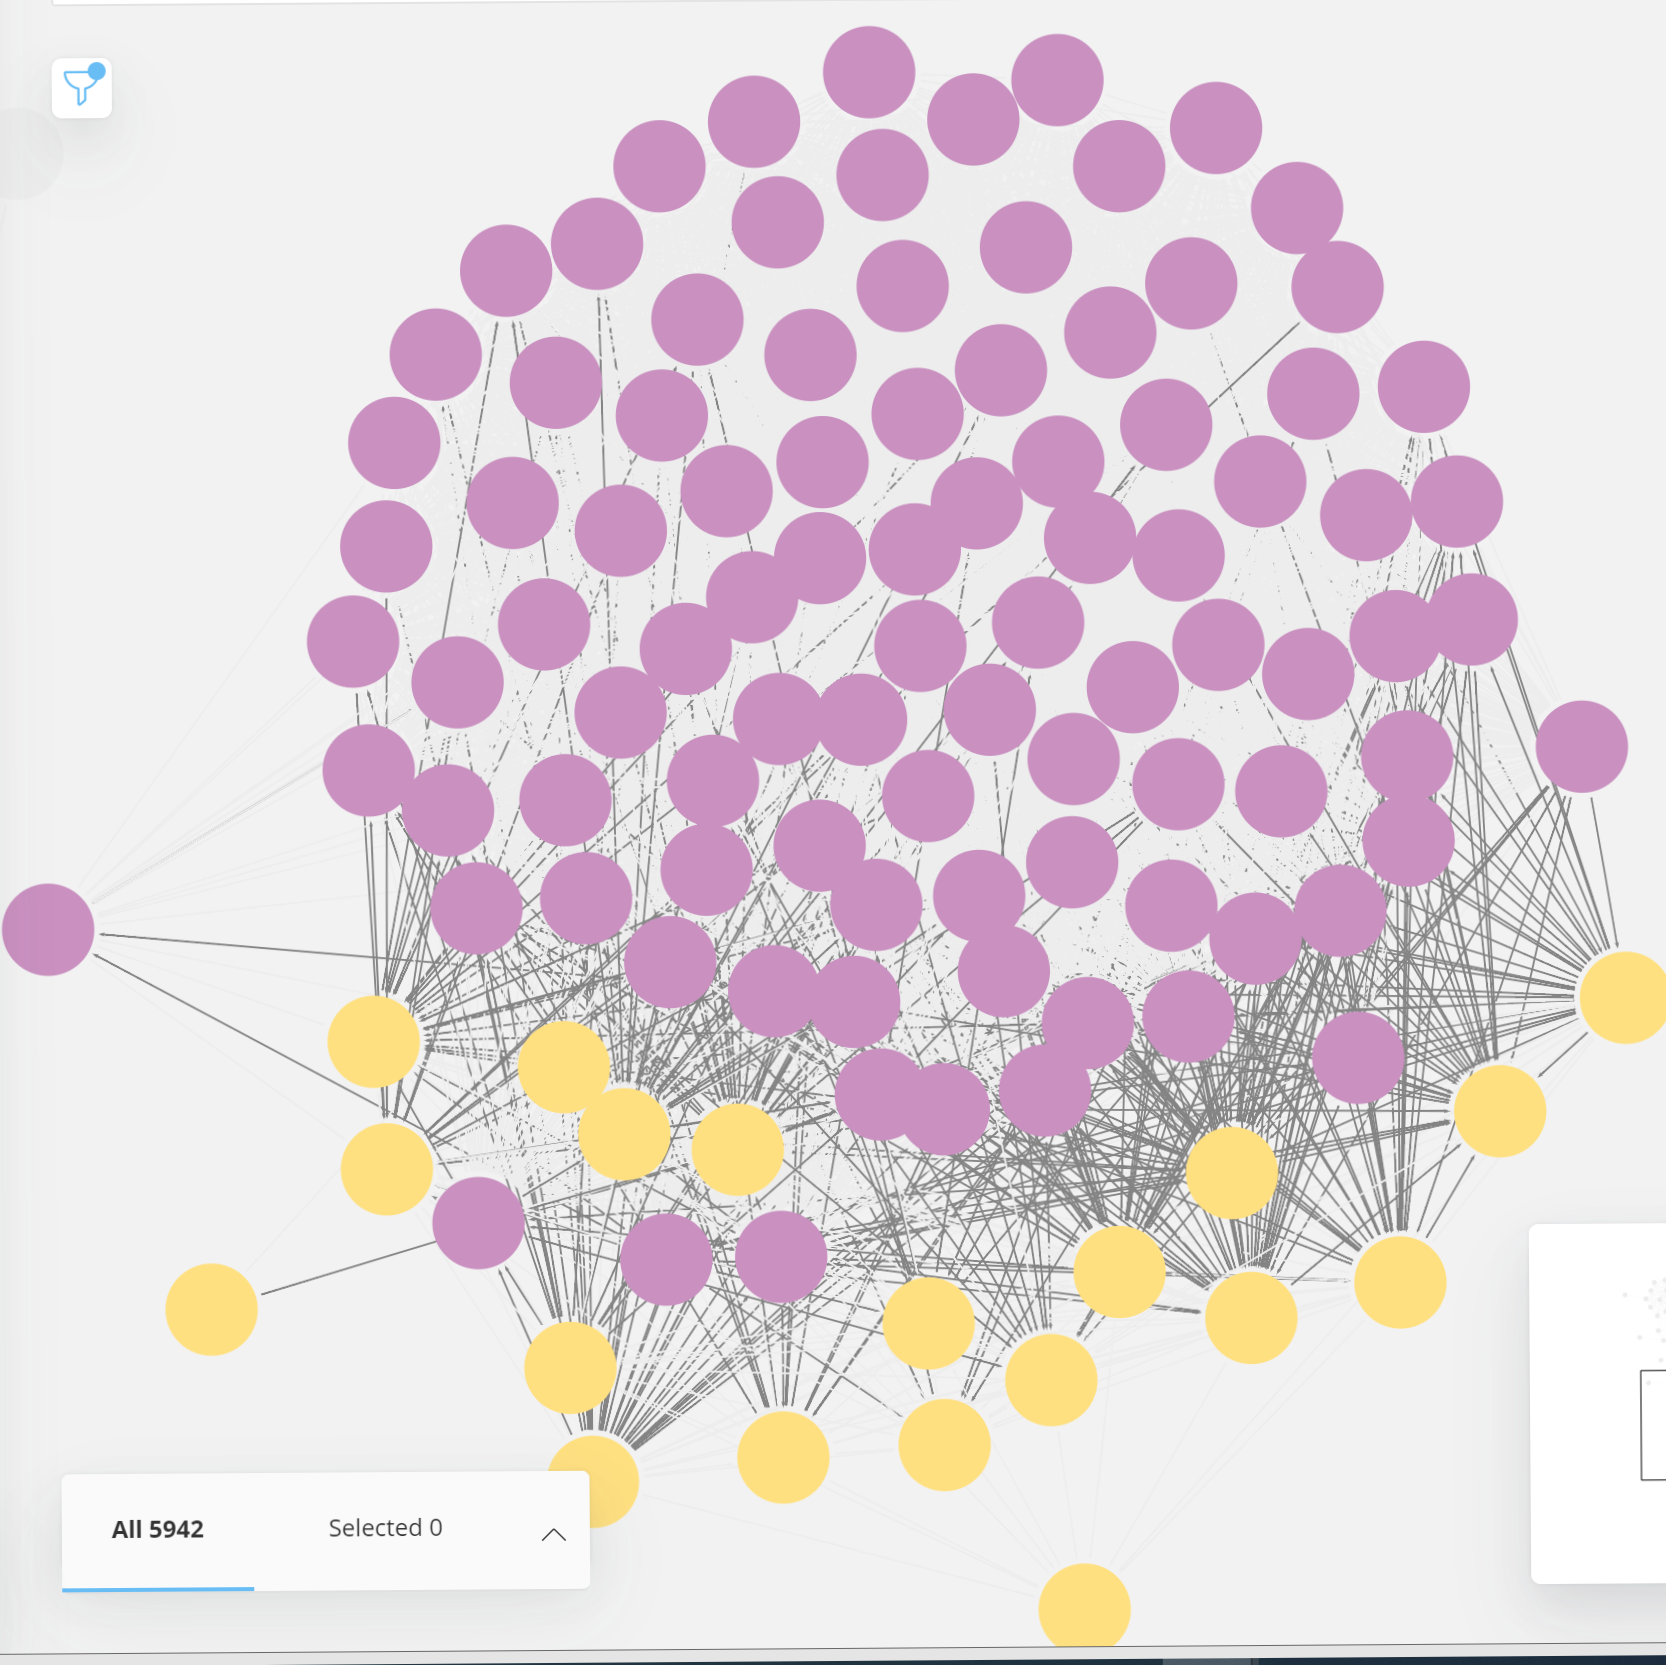
\includegraphics[]{img/only3.png}}
%     \caption{ Graph with edges of Type 3}
%     \label{subfig:ab3}
%   \end{subfigure}
%     \caption{Ablation study on Relational sentence graph. {Violet nodes} are non-biased, {Yellow nodes} are biased.}
%     \label{fig:ablation}
%   \end{figure*}
  

\begin{table*}[htbp]
  \centering 
    \begin{tabular}{p{4em}p{6em}p{6em}p{6em}p{6em}p{6em}p{6em}p{6em}}
    \toprule
         \textbf{Variant} & \textbf{MultiCTX} & \textbf{CSE + BiLSTM} & \textbf{Discourse relationship } & \textbf{Semantic similarity} & \textbf{Event-context} & \textbf{Neighborhood-context}  &  \textbf{w/o Entity continuation} \\\midrule
        %  w/ or w/o &  &  &  only  & only   & w/o  & only &  w/o \\ \midrule
        %  \multicolumn{5}{l}{$^${*} All results are implemented or reproduced by ourselves except for the second EvCIM record}
        %  without &  &  & Semantic similarity &  & Adjacent sentences &  &  Entity continuation  \\ \hline
       Edge types &  all=[1,2]$^{*}$,3,4  & No graph & [1,2],3 & 4  & 3,4 &  [1,2] & [1,2],4\\\hline
      %  Context level &  Neighborhood + Event &  & Neighborhood + Event & Event  & Event &  Neighborhood & Neighborhood + Event \\\hline
    Precision &    $47.78 \pm 0.94$   &  $48.53 \pm 0.73$ &  $47.43 \pm 0.96$ &    $47.16 \pm 0.27$   &  $47.07\pm 0.99$ &  $47.18 \pm 1.08$     &  $47.56 \pm 0.62$       \\
    \hline
    Recall &   $44.50 \pm 0.65$    &   $41.98\pm 0.36$  & $44.39\pm 0.84$  &    $43.47\pm 0.38$ & $44.64\pm 0.37$  & $44.01\pm 0.91$  &      $43.72\pm 0.76$   \\
    \hline
    F1    &  $46.08\pm0.21$  & $45.01 \pm 0.26 $  &   $45.85\pm0.35$    &  $45.24\pm0.18$        & $45.81\pm0.42 $     & $45.53\pm0.29$   &  $45.55\pm0.34$\\
    \bottomrule
    \multicolumn{8}{l}{$^{*}$  Type 1 together with Type 2 represents the Neighborhood-level context so we treat them as a whole in the ablation study.} \\
    \end{tabular}%
      \caption{Ablation study on different types of edges in SSGAT. Mean and standard deviation across 5 seeds are reported.}
  \label{tab:ablation}%
\end{table*}%


  
Table \ref{tab:ablation} shows the ablation results. We can conclude that, 

\begin{itemize}
    \item \textbf{Context information transfers via edges in graph is better than via cells in BiLSTM. }
    
    All variants with graphs have better F1 score than the model without graph (CSE+BiLSTM, F1=45.01). 
    
    Figure \ref{fig:ablation} shows graphs with different edges in our ablation study using a subgraph of one event. {Violet nodes} are non-biased sentences, {Yellow nodes} are biased sentences.
    
    \item \textbf{Discourse relationship contributes more than the semantic similarity to SSGAT.} SSGAT with only discourse relationships (F1=45.85) still has close performance to the full MultiCTX, while SSGAT with only semantic similarity edges (F1=45.25) suffers a considerable decrease in its performance. Note that the semantic similarity is calculated based on CSEs, so SSGAT with only such edges didn't add much extra information but may introduce duplication. It can be explained by Figure \ref{subfig:ab4}: connections are mostly within non-based words while inter-communication between biased/non biased nodes are more frequent in Figure \ref{subfig:ab123}.
    
    % edges of Therefore, edges connected by semantic similarity and by discourse relationships may overlap partially.
    
    % Note that the semantic similarity is calculated based on CSEs, and CSEs are learnt from article and event contexts encoded by triplets. Therefore, edges connected by semantic similarity and by discourse relationships may overlap partially.

    \item \textbf{Event-level context is more important than the neighborhood-level context.} While they are both important according to our results, global event-level context contributes more than local neighborhood-level context. SSGAT with only adjacent sentences (Type 1,2) obtains F1=45.53 and with only Type 3,4 gets F1=45.81. The result is intuitive because edges of type 3,4 not only include adjacent sentences within article, but also extend to the whole event. We can also see the rare presence of edges of Type 1,2 in Figure \ref{subfig:ab12} compared with the closely linked graph in Figure  \ref{subfig:ab34}.

    \item \textbf{Adjacent sentences encoded by graph better interprets context information than brute-force PLMs.} In terms of neighborhood-level context, our SSGAT beats WinSSC by increasing massively the F1 score from F1=37.58 (Table \ref{tab:res}) to F1=45.53. 
    
    
    \item \textbf{Entity continuation is the most important edge type.} Among three ablation experiments removing respectively edges of Type 4 (F1=45.85), Type 1,2 (F1=45.81) and Type 3 (F1=45.55), the last one without Type 3 (entity continuation) suffers the largest performance drop. It suggests that entity continuation, or, coreference is the most important relation in our setting.
    We can clearly see that Type 3 edges are the main reason for inter-class communication from Figure \ref{subfig:ab3}.

\end{itemize}



\begin{table*}[htbp]
  \centering 
    \begin{tabular}{p{4em}p{6em}p{6em}p{6em}p{6em}p{6em}p{6em}p{6em}}
    \toprule
         \textbf{Variant} & \textbf{MultiCTX} & \textbf{CSE + BiLSTM} & \textbf{Discourse relationship } & \textbf{Semantic similarity} & \textbf{Event-context} & \textbf{Neighborhood-context}  &  \textbf{w/o Entity continuation} \\\midrule
        %  w/ or w/o &  &  &  only  & only   & w/o  & only &  w/o \\ \midrule
        %  \multicolumn{5}{l}{$^${*} All results are implemented or reproduced by ourselves except for the second EvCIM record}
        %  without &  &  & Semantic similarity &  & Adjacent sentences &  &  Entity continuation  \\ \hline
       Edge types &  all=[1,2]$^{*}$,3,4  & No graph & [1,2],3 & 4  & 3,4 &  [1,2] & [1,2],4\\\hline
      %  Context level &  Neighborhood + Event &  & Neighborhood + Event & Event  & Event &  Neighborhood & Neighborhood + Event \\\hline
    Precision &    $47.78 \pm 0.94$   &  $48.53 \pm 0.73$ &  $47.43 \pm 0.96$ &    $47.16 \pm 0.27$   &  $47.07\pm 0.99$ &  $47.18 \pm 1.08$     &  $47.56 \pm 0.62$       \\
    \hline
    Recall &   $44.50 \pm 0.65$    &   $41.98\pm 0.36$  & $44.39\pm 0.84$  &    $43.47\pm 0.38$ & $44.64\pm 0.37$  & $44.01\pm 0.91$  &      $43.72\pm 0.76$   \\
    \hline
    F1    &  $46.08\pm0.21$  & $45.01 \pm 0.26 $  &   $45.85\pm0.35$    &  $45.24\pm0.18$        & $45.81\pm0.42 $     & $45.53\pm0.29$   &  $45.55\pm0.34$\\
    \bottomrule
    \multicolumn{8}{l}{$^{*}$  Type 1 together with Type 2 represents the Neighborhood-level context so we treat them as a whole in the ablation study.} \\
    \end{tabular}%
      \caption{Ablation study on different types of edges in SSGAT. Mean and standard deviation across 5 seeds are reported.}
  \label{tab:ablation}%
\end{table*}%

% \begin{table*}[htbp]
%   \centering
%     \begin{tabular}{p{4em}p{5em}p{6em}p{5em}p{5em}p{5em}p{6em}p{6em}}
%     \toprule
%          \textbf{Variant} & \textbf{MultiCTX} & \textbf{CSE + BiLSTM} & \textbf{Discourse relationship } & \textbf{Semantic similarity} & \textbf{Event-context} & \textbf{Neighborhood-context}  &  \textbf{w/o Entity continuation} \\\midrule
%         %  w/ or w/o &  &  &  only  & only   & w/o  & only &  w/o \\ \midrule
%         %  \multicolumn{5}{l}{$^${*} All results are implemented or reproduced by ourselves except for the second EvCIM record}
%         %  without &  &  & Semantic similarity &  & Adjacent sentences &  &  Entity continuation  \\ \hline
%       Edge types &  1,2,3,4  & No graph & 1,2,3 & 4  & 3,4 &  1,2 & 1,2,4\\\hline
%       %  Context level &  Neighborhood + Event &  & Neighborhood + Event & Event  & Event &  Neighborhood & Neighborhood + Event \\\hline
%     Precision &    $47.78 \pm 0.94$   &  $48.53 \pm 0.73$ &  $47.43 \pm 0.96$ &    $47.16 \pm 0.27$   &  $47.07\pm 0.99$ &  $47.18 \pm 1.08$     &  $47.56 \pm 0.62$       \\
%     \hline
%     Recall &   $44.50 \pm 0.65$    &   $41.98\pm 0.36$  & $44.39\pm 0.84$  &    $43.47\pm 0.38$ & $44.64\pm 0.37$  & $44.01\pm 0.91$  &      $43.72\pm 0.76$   \\
%     \hline
%     F1    &  $46.08\pm0.21$  & $45.01 \pm 0.26 $  &   $45.85\pm0.35$    &  $45.24\pm0.18$        & $45.81\pm0.42 $     & $45.53\pm0.29$   &  $45.55\pm0.34$\\
%     \bottomrule
%     \end{tabular}%
%       \caption{Ablation study on different types of edges in SSGAT. Mean and standard deviation across 5 seeds are reported.}
%   \label{tab:ablation}%
% \end{table*}%
